% --------------------------------------------
%		CAPITOLO 5
%---------------------------------------------

\chapter{TJ-Monopix2 characterization} \label{ch:TJ2}

In this chapter we will go through the main features of TJ-Monopix2 designed to address efficiency degradation after irradiation, one of the main issues of its predecessor TJ-Monopix1. The characterization of the chip is crucial in the VTX upgrade program and in the design of the next OBELIX chip.\\
The chip W14R12, which is one of the sensors tested during the first Test Beam (TB) campaign in Desy (July 2022) has been fully characterized in Pisa and in particular several aspects have been analyzed, among which:

\begin{enumerate}
\item TOT calibration by internal charge injection;
\item characterization with radioactive sources and absolute calibration;
\item systematic study of different registers' settings in order to operate the chip at low thresholds;
\item investigation of an important issue with cross-talk, due to digital signal from the readout, discovered trying to operate the matrix at low threshold (below 250 $e^{-}$).
\end{enumerate}

This detailed characterization returned crucial results (1, 2) for the Test Beam data reconstruction and the simulations of the upgraded VTX detector with CMOS MAPS devices. Furthermore the optimization of the registers to reduce the operating threshold was very useful for the preparation of the next TB (July 2023) campaign with irradiated sensors.


%FOTO TJ MONOPIX 2
\begin{figure}[h!]
\centering
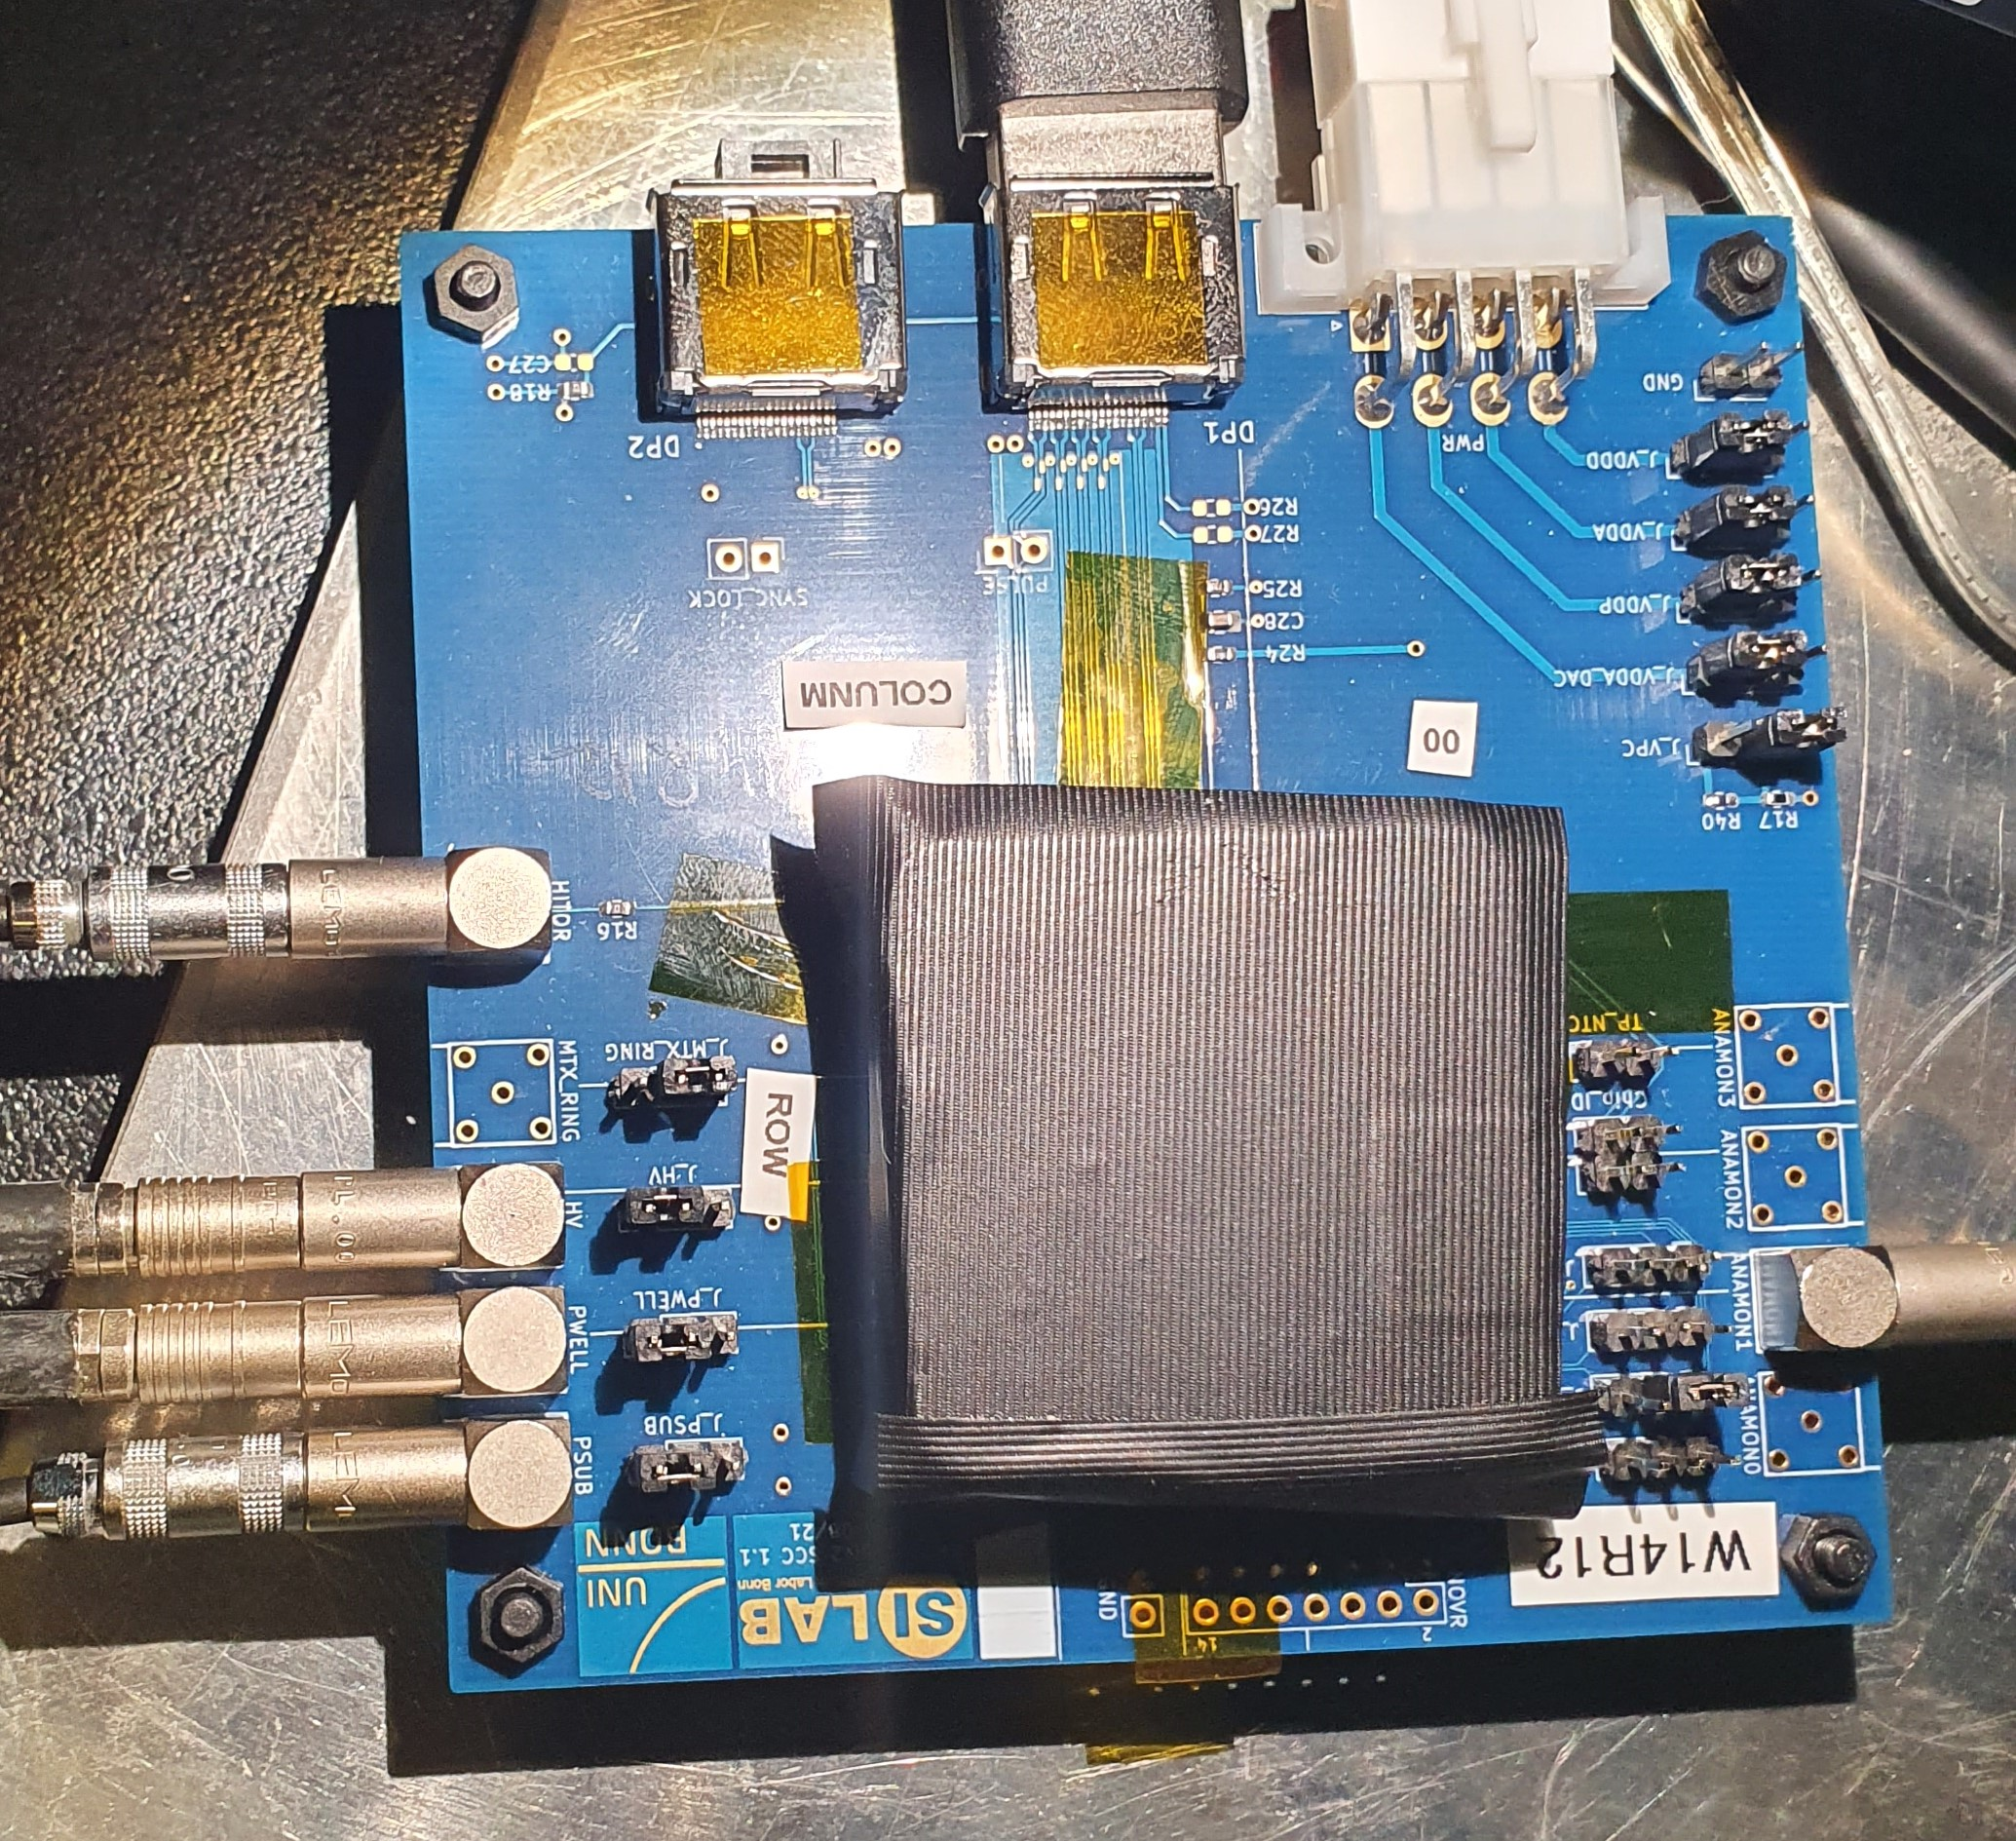
\includegraphics[scale=.08]{W14R12}
\caption{The W14R12 chip tested during the Test Beam in Desy.}
\label{fig:w14r12}
\end{figure}


% --------------------------------------------
%	5.1 MATRIX AND FLAVORS
%---------------------------------------------

\section{Matrix and flavors}


TJ-Monopix2 is the next generation small collection electrode DMAPS prototype in TowerJazz 180 nm. The need to create a sensor capable to mantain high efficiency even after irradiation, required improvements compared to TJ-Monopix1 in two important fields: a lower operating threshold to keep a good efficiency with the reduced charge collected after irradiation and smaller pixel pitch to increase charge collection efficiency all over its area, expecially in the corners.\\

To achieve these goals, a different in-pixel front-end circuit was implemented and a lot of efforts have been focused on optimizing pixel layout in order to reduce its size, which has been decreased from \numproduct{36 x 40}~\unit{\micro m^{2}} in TJ-Monopix1 to \numproduct{33.04 x 33.04}~\unit{\micro m^{2}} (pixel \textit{pitch}). The pixel dimensions are critical to accomplish faster charge collection across all active area, increasing the lateral electric field (\autoref{sec:TJ}). For this reason it was necessary a special effort to design and create a smaller pixel but still adequate to embody the full digital readout. All of this required to work at the technology density limit and also to study for further modifications at the circuit design.

In order to operate with a lower threshold TJ-Monopix2 incorporates an improved front-end circuit that reduces the noise by $\approx$ 40\% and the threshold dispersion by about 80-90\% with respect to TJ-Monopix1. Furthermore, in-pixel threshold tuning has been integrated in order to achieve a more uniform threshold distribution across the pixel matrix, particularly after irradiation. As a result of these improvements, the operating threshold was expected to be at $\approx$ 100 $e^{-}$, three times lower than in TJ-Monopix1.


%-----------------------------------------------------------------------------------------------

\subsection{Flavors} \label{sec:flavors}

The protype is a \numproduct{2 x 2}~\unit{cm^{2}} pixel matrix which consists of \numproduct{512 x 512} pixels. The total active area is approximately \SI{286}{mm^{2}} and it is \SI{300}{\micro m} thick.


As we can see in~\autoref{fig:tj2matrix}, the matrix is divided in four sectors, named \textbf{flavors} that implement different variation of the front-end circuit. In the first two flavors the collection electrode is DC-coupled directly with the readout electronics,  the continuous baseline reset is implemented by a forward bias diode and they differ for the pre-amplifier circuit design. The second flavor indeed, named \textbf{Cascode FE}, includes an extra-cascode transistor that increases the pre-amplifier gain which in turn leads to a 50\% reduction of the threshold dispersion compared to the first flavor, the \textbf{Normal FE}. The other two flavors consist of AC-coupled pixels (through a metal-oxide-metal MOM capacitor) and in particular, the \textbf{HV-Cascode FE} also incorporates the aforementioned pre-amplifier variation. AC-coupling allows to apply an high positive bias voltage (HV stands for High Voltage) to the collection electrode which potentially enlarges the depleted region, but at the same time it also causes signal losses mainly due to the additional parasitic capacitance introduced at the sensitive input node.\\


\begin{figure}[h!]
\centering
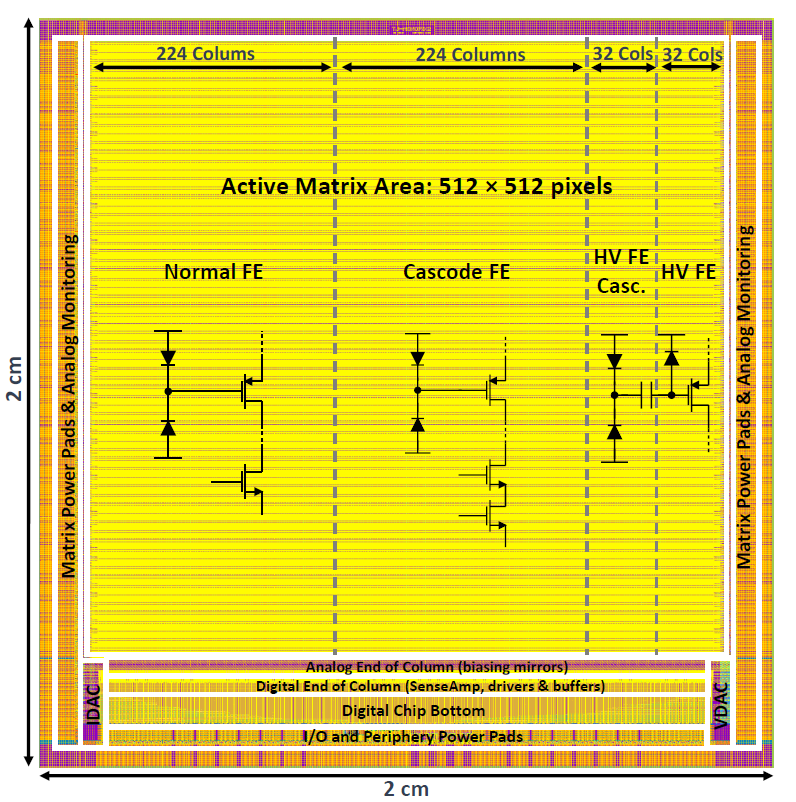
\includegraphics[scale=.5]{Matrix}
\caption{The layout of the TJ-Monopix2 prototype divided in four different flavors: \textbf{Normal}, \textbf{Cascode}, \textbf{HV-Cascode} and \textbf{HV FE}.}
\label{fig:tj2matrix}
\end{figure}


%-----------------------------------------------------------------------------------------------%

\subsection{Pixel design}

The \numproduct{2 x 2} pixel core layout, shown in~\autoref{fig:tj2core}, is fully optimized and is designed in order to share as much features as possible between the four pixels. The analog area incorporates the front-end circuit, the 3-bit threshold tuning DAC and the pixel configuration registers. The digital region is composed by the 7-bit LE and TE memory (14 SRAM cells per pixel), the 10 bit address ROM (2 bit for the pixel position inside the core and 8 for the group address) and the readout control logic. 

\begin{figure}[h!]
\centering
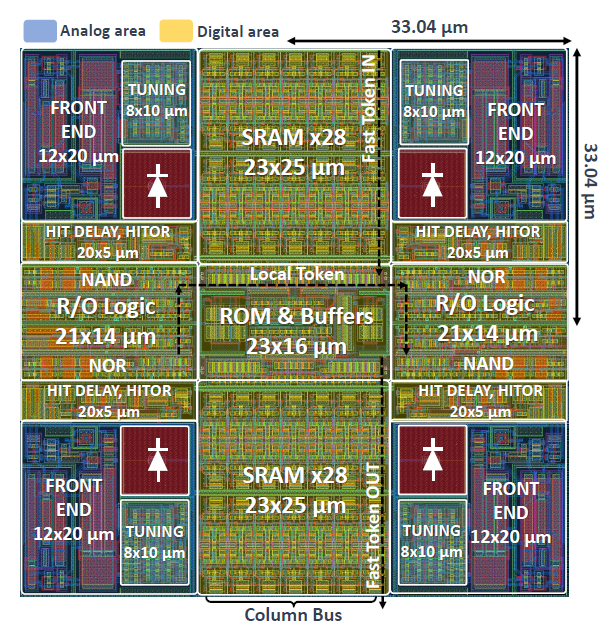
\includegraphics[scale=.5]{pixel_core}
\caption{Layout of a TJ-Monopix2 \numproduct{2 x 2} pixel core. In blue the analog area and in yellow the digital one.}
\label{fig:tj2core}
\end{figure}


%-----------------------------------------------------------------------------------------------%

\subsubsection{Improved front-end circuit design}\label{sec:improved_circuit}

As we have seen above, there are two variations of the front-end circuit (\autoref{fig:tj2_circuit}), such as \textit{normal} and \textit{cascode} type. The latter in particular includes an extra cascode transistor which increases the pre-amplifier gain and consequently reduces the threshold dispersion.\\
Moreover in TJ-Monopix2 it was preferred to incorporate a simple diode to reset the input node instead of a PMOS transistor, which was the techonology implemented in TJ- Monopix1. A side effect of this choice is that the relationship between charge injected and the ToT of the detected signal is not linear anymore, because the diode is a not linear element and its discharge rate also depends on the collected charge. Indeed in the following analysis it was necessary to fit the ToT trend with a more complex function. But at the same time, the advantages are its simplicity ($p^{+}$ diffusion within the n-well collection electrode) and also the fact that it allows to increase radiation tolerance to Total Ionizing Dose (TID) effects, which was one of the key working area in the upgrade of the sensor.


\begin{figure}[h!]
\centering
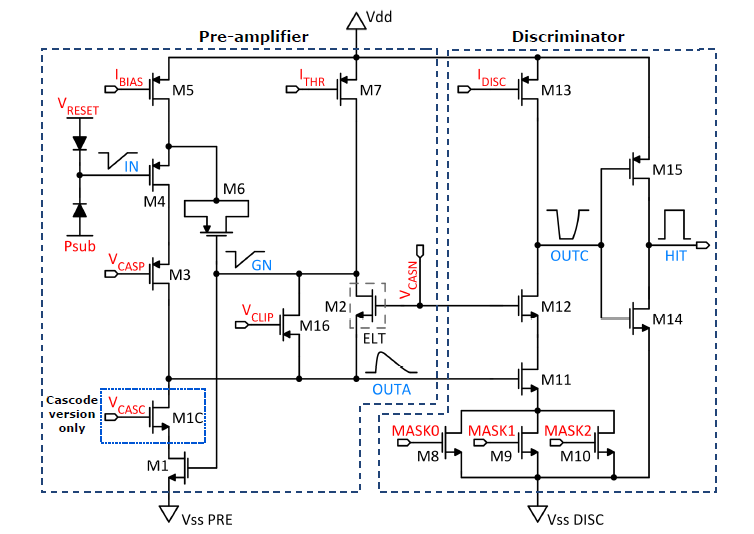
\includegraphics[scale=.7]{tj2-circuit}
\caption{Schematic of the improved front-end circuit and its variation (extra-cascode transistor) in TJ-Monopix2.}
\label{fig:tj2_circuit}
\end{figure}


In the last two AC-coupled flavors are implemented the same improvements, but here the different coupling provokes an important loss in the collected charge, as verified during the testing phase of TJ-Monopix1 (50\% losses), due at most to additional parassitic capacitances. Thus a lot of efforts have been made to improve this aspect, working on the coupling capacitor values. A signal loss of 41.5\% has been reached in TJ-Monopix2, which is a relevant enhancement with respect to its predecessor.




% --------------------------------------------
%	5.2 THRESHOLD AND NOISE
%---------------------------------------------

\section{Threshold and noise} \label{thresh_noise}


\textbf{Explain here what are NOISE, THR and THR dispersion, and why they are important figure of merit for the operation.} 

see for example Eleonora's thesis sec 4.1.1. 


To measure the threshold and noise of the whole matrix, the response of each pixel has been characterized by means of the internal charge injection. \\

\subsection{Injection circuit} \label{inj_circuit_subsection}

The hit injection circuit included in TJ-Monopix2 is similar to the one of TJ-Monopix1. 
It allows to produce artificial hits on each pixel through an injection capacitance \textbf{$C_{inj}$} connected at the collection electrode. The injected charge is proportional to the injection voltage pulse amplitude: $Q_{inj} = C_{inj} \cdot \Delta V_{inj}$. The injection pulse is set by two registers ''\textbf{$V_{L}$}'' and ''\textbf{$V_{H}$}'', with $\Delta V_{inj}$ = \textbf{$V_{H}-V_{L}$}, and the minimum injection step is given by the DAC resolution, with the \textit{Least Significant Bit} (LSB) = 7.03 mV. 

The injected signal is then often expressed in DAC units $Q_{inj}(DAC)$ and can be converted to electrons using the design value of the injection capacitance \textbf{$C_{inj}= 230\ aF$}, the same for the all the FEs implemented.  
The nominal conversion factor $K$ from DAC to $e^{-}$ corresponds to the injected charge given by a voltage step of 1 DAC: 

\begin{equation}
\small
K = C_{inj} \cdot LSB = \frac{230 \, aF}{q_{{e}^{-}}} \cdot 7.03 \frac{mV}{DAC}= 1.4375 \frac{e^{-}}{mV} \cdot 7.03 \frac{mV}{DAC} \approx 10.1 \frac{e^{-}}{DAC}  
\label{eq:conversion_factor}
\end{equation}


An absolute calibration of the conversion factor $K$ (i.e. of the injection capacitance $C_{inj}$) has been also performed using radioactive sources, as explained in~\autoref{sec:source_ana}, obtaining results in agreement within 10$\%$ from the design value. 

The conversion factor of~\autoref{eq:conversion_factor} has been used to convert the information of the injected charge from DAC unit to electrons unit, useful for further analysis.
\\
The response of each pixel to internal injection has been measured to extract their threshold and noise with the \textit{s-curve method} explained in the next section. 
The four flavors have been separately analyzed to be able to study their main differences concerning their performance and features. 


%--------------------------------------------------------------------
\subsection{S-Curve method} \label{sec:threshold_subsection}

The response of the pixels is measured injecting different amounts of charge into the pixel a given number of times and recording the amount of registered hits (i.e. the signal is above the discriminator threshold). For each value of the input signal we measure the occupancy, or hit probability, as the fraction of events where the pixel has registered a hit. This occupancy has the typical S-curve shape shown in~\autoref{fig:ex_scurve} as an example. 

As the injected signal passes the discriminator threshold the pixel starts to register some hits, finally reaching a plateau corresponding to the total number of injected events. This behaviour produces a step function smeared by the fluctuation on the input signal due to the noise.  
The threshold of the pixel corresponds to the injected signal  that gives 50\% occupancy, while the noise influences the slope of the S-curve.  

Assuming a gaussian noise distribution the S-curve can be fit with the \textit{Cumulative Distribution Function (CDF)}:

\begin{equation}
 CDF(x,\mu,\sigma) = \frac{1}{2} \cdot \bigg(1 + \textit{erf}\bigg(\frac{x-\mu}{\sigma \sqrt{2}}\bigg)\bigg)
\end{equation}

where ''\textit{erf}'' is the Gauss error function, $x$ is the injected signal, $\mu$ and $\sigma$ are respectively the threshold and noise of the pixel.  \\

This method allows to measure the noise and the threshold of all pixels and also the threshold dispersion across an entire FE.

\begin{figure}
\centering
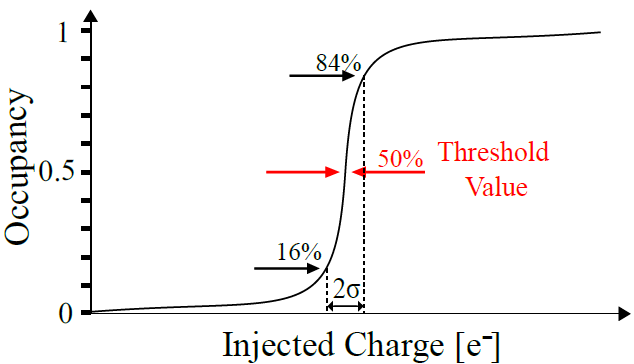
\includegraphics[scale=.6]{scurve_ex2}
\caption{An example of the S-Curve fitted by the CDF to evaluate threshold and noise.}
\label{fig:ex_scurve}
\end{figure}

In the following sections are reported the results of this study for the four flavors of the matrix. The injected signal was varied, with the corresponding voltage injection registers ''\textbf{VL,VH}'' , from 0 to 140 DAC, corresponding to a charge of $\approx$ 1400 $e^{-}$, adopting the conversion factor in~\autoref{eq:conversion_factor} .


\subsubsection{Normal FE}

The first flavor of the matrix is the \textbf{Normal FE}, which consists of 512 rows and 224 columns for a total of 114.688 pixels. The chip registers have been set with the same values used during the Test Beam at Desy (July 2022) which are different for the DC and AC-coupling case. They are called for simplicity ''\textbf{GOE settings}'' and they are reported in~\autoref{tab:tb_settings}, where the different biasing voltages used to power up the chip are also added.

\begin{table}[h!]
\centering
%\begin{tabular}{>{\columncolor{ProcessBlue!60}} C{3.2cm}|C{3.7cm}|C{3.5cm}}
\begin{tabular}{C{3.2cm}|C{3.7cm}|C{3.5cm}}
%\rowcolor{lightgray}
Registers & Normal/Cascode FE ($P_{SUB}$/$P_{WELL}$ = -3 V) & HV/HV-Cascode FE ($P_{SUB}$/$P_{WELL}$ = 0 V, HV = +5 V)\\[2ex]
\hline
\hline
$I_{THR}$ & 64 & 30\\[0.5ex]
\hline
$I_{BIAS}$ & 50 & 60\\
\hline
$V_{RESET}$ & 143 & 100\\
\hline
$I_{CASN}$ & 0 & 8\\
\hline
$I_{DB}$ & 100 & 100\\
\hline
$I_{TUNE}$ & 53 & 53\\
\hline
\hline
\end{tabular}
\caption{Settings of the main registers used for all flavors (W14R12 chip) during the Test Beam in Desy.}
\label{tab:tb_settings}
\end{table}


\begin{figure}[h!]
\centering
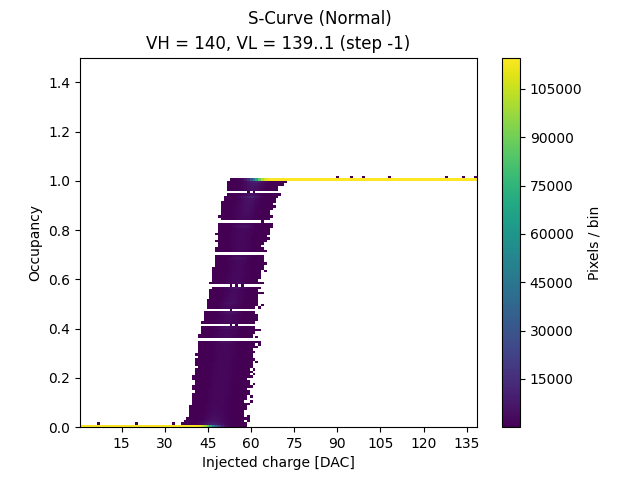
\includegraphics[scale=.6]{all_norm_thscan_140}
\caption{S-curves of all pixels of the Normal FE with a maximum injection pulse of 140 DAC.}
\label{fig:norm_scurve_140}
\end{figure}


In~\autoref{fig:norm_scurve_140} are plotted all the s-curves of the all Normal flavor pixels. The width of the figure is a first indication of the threshold dispersion of the whole flavor.\\

The threshold and noise distributions measured by the s-curve method, have been fitted with a gaussian distribution and they are shown in~\autoref{fig:thdist_norm} with their maps, too.

\begin{figure}[h!]
\centering
\subfigure[Threshold distribution]
{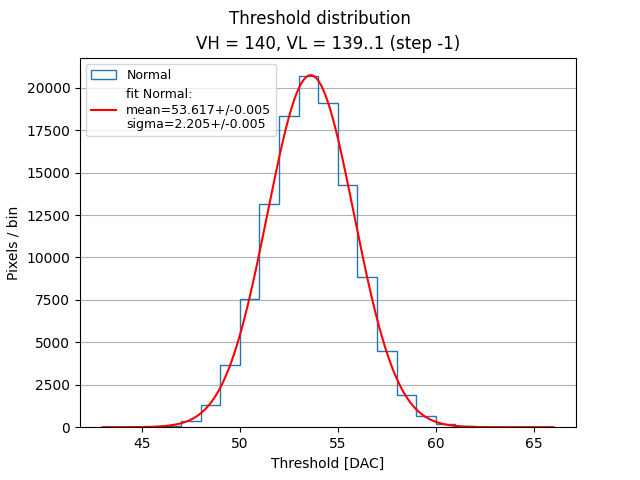
\includegraphics[scale=0.35]{all_norm_thdist_140}}\quad
\subfigure[Threshold map]
{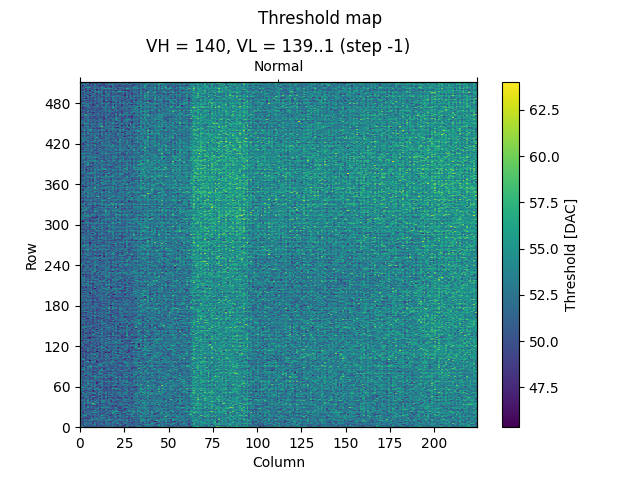
\includegraphics[scale=0.37]{threshold_map_norm_140}}\\
\subfigure[Noise distribution]
{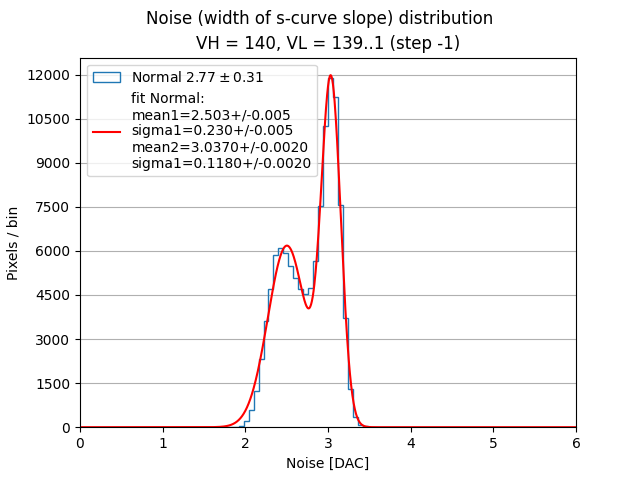
\includegraphics[scale=0.35]{Noise_hist_norm_140_fit}}\quad
\subfigure[Noise map]
{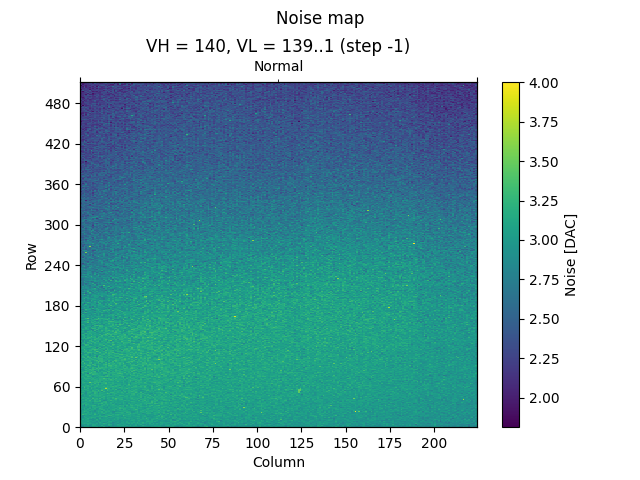
\includegraphics[scale=0.37]{Noise_map_norm_140}}\\
\caption{Normal FE.}
\label{fig:thdist_norm}
\end{figure}



\subsubsection{Cascode FE}

\textbf{Cascode FE} is the second flavor and, like the previous one, it consists of 512 rows and 224 columns for a number of total pixels equal to 114.688. For this flavor the same procedure of Normale FE has been followed and the same registers' values (\autoref{tab:tb_settings}) have been used.
In~\autoref{fig:casc_scurve140} the s-curves of all pixels are shown.

\begin{figure}[h!]
\centering
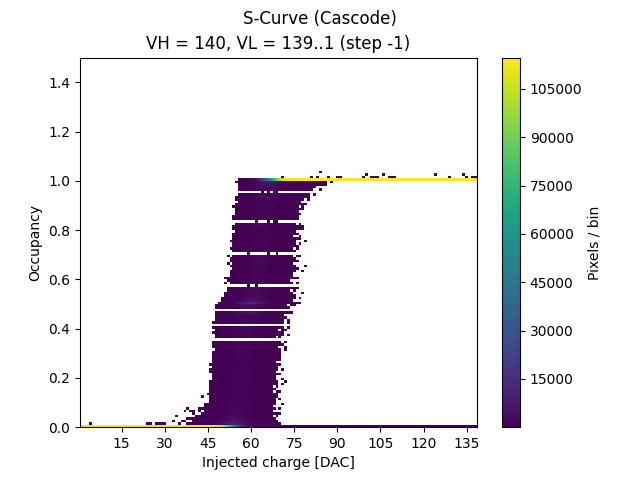
\includegraphics[scale=.5]{all_casc_thscan_140}
\caption{S-curves of all pixels in the \textbf{Cascode} flavor with a maximum injection pulse of 140 DAC.}
\label{fig:casc_scurve140}
\end{figure}

The maps and the fit of the threshold and noise distributions instead, are shown in~\autoref{fig:thdist_casc}.


\begin{figure}[h!]
\centering
\subfigure[Threshold distribution]
{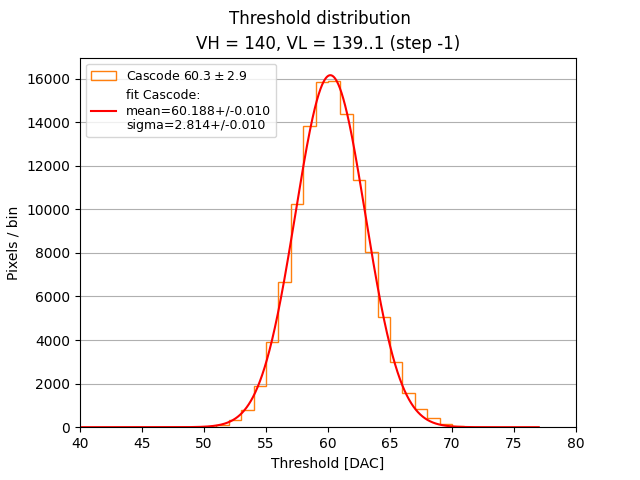
\includegraphics[scale=0.35]{all_casc_thdist_140}}\quad
\subfigure[Threshold map]
{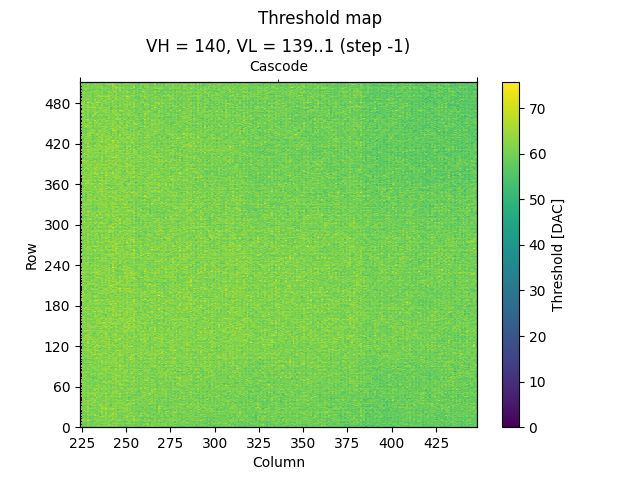
\includegraphics[scale=0.37]{threshold_map_casc_140}}\\
\subfigure[Noise distribution]
{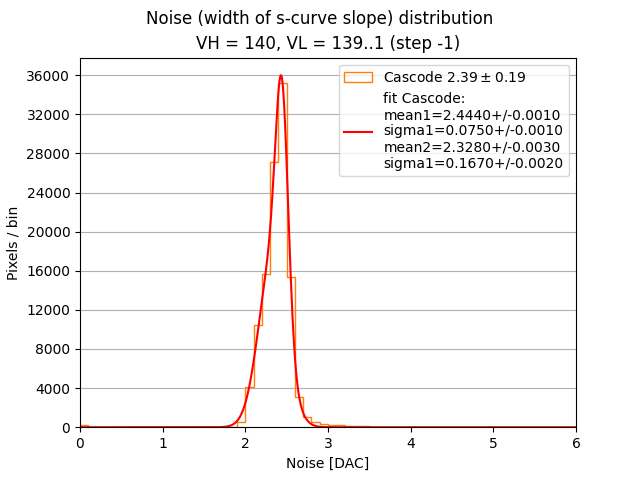
\includegraphics[scale=0.35]{Noise_hist_casc_140_fit}}\quad
\subfigure[Noise map]
{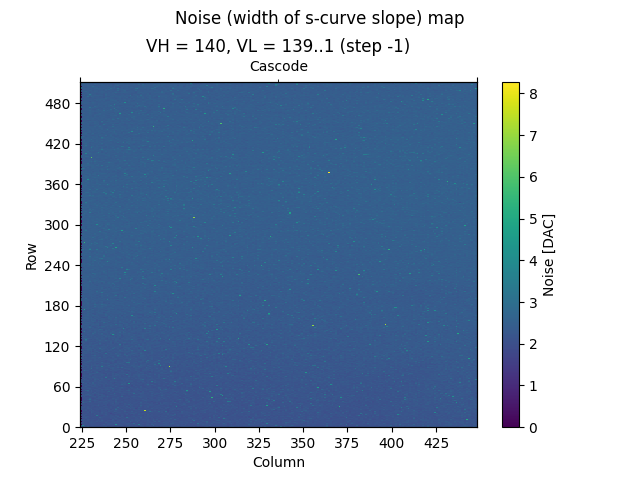
\includegraphics[scale=0.37]{Noise_map_casc_140}}\\
\caption{Cascode FE.}
\label{fig:thdist_casc}
\end{figure}



\subsubsection{HV-Cascode FE}


The third flavor is \textbf{HV-Cascode FE} and it is composed by 512 rows and 32 columns for a total number of pixel equal to 16384. Also for these last two flavors, the main chip registers are set with the same values tested and used during the Test Beam (but different from those used for the first two flavors). They are reported in~\autoref{tab:tb_settings} .

As we can see from the plot of the alle s-curves in~\autoref{fig:hvc_scurve_140}, with this choice of registers there were a lot of ''hot'' pixels with occupancy > 1, but at this stage of measurements they were not masked.
These hot pixels with occupancy > 1, register more hits than the number of injected events. This behaviour seems to indicate that they are stimulated, not by the charge injection, but by some other input, due to ''cross-talk'', active during the readout of the matrix. The origin of the hot pixel and cross-talk was carefully investigated later (see~\autoref{sec:xtalk})
.

\begin{figure}[h!]
\centering
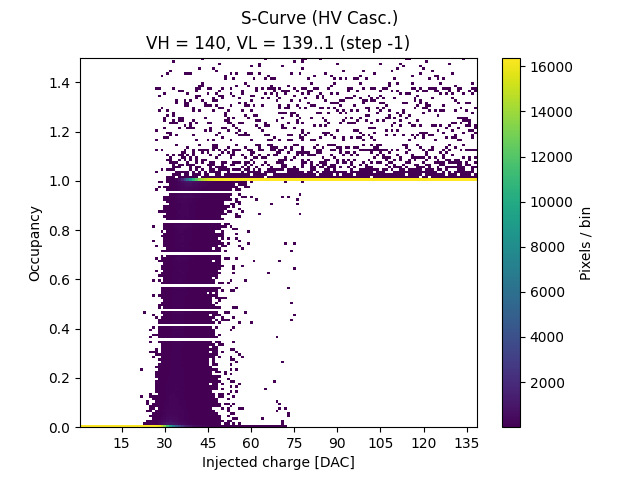
\includegraphics[scale=.5]{all_HVc_thscan_140}
\caption{S-curves of all pixels in \textbf{HV Cascode} flavor with a maximum injection pulse of 140 DAC.}
\label{fig:hvc_scurve_140}
\end{figure}

In~\autoref{fig:thdist_hvc} are shown the fit of the threshold and noise distributions.

\begin{figure}[h!]
\centering
\subfigure[Threshold distribution]
{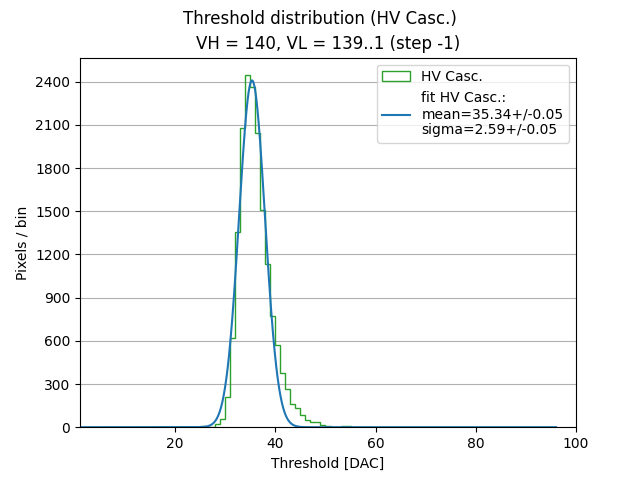
\includegraphics[scale=0.35]{all_HVc_thdist_140}}\quad
\subfigure[Noise distribution]
{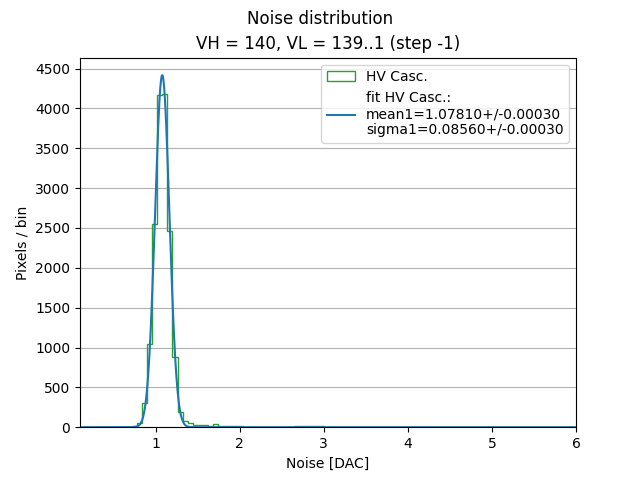
\includegraphics[scale=0.37]{Noise_hist_HV Casc._140_fit}}\\
\caption{HV Cascode FE.}
\label{fig:thdist_hvc}
\end{figure}


\subsubsection{HV-Normal FE}\label{sec:first_xtalk}

The fourth and last flavor is the \textbf{HV-Normal FE} which has the same layout of the previous FE. The main registers have been set with the values reported in~\autoref{tab:tb_settings}.
The s-curves of all pixel in this flavor are shown in~\autoref{fig:hv_scurve_140} and we can notice that there were some hot pixels unmasked.
Moreover the last 16 columns were not working (visible in the maps in~\autoref{fig:HVs_maps}) and as a matter of fact they had return a peak of threshold near the value 0, which is excluded from the threshold distributions plots.

Therefore in this part of the matrix, the real number of pixel studied was 8192, half of the total.


\begin{figure}[h!]
\centering
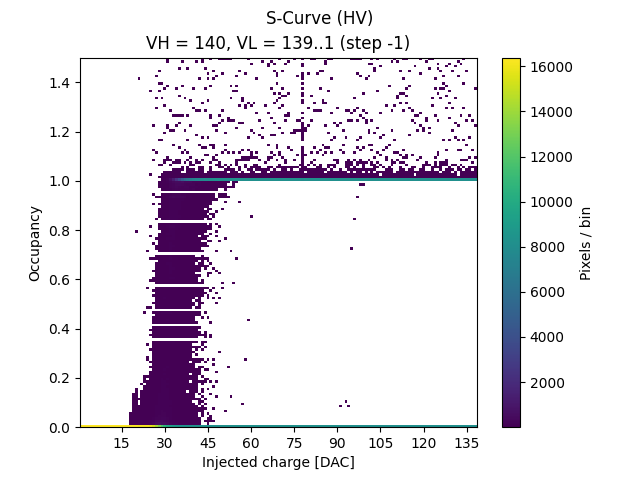
\includegraphics[scale=.5]{all_HV_thscan_140}
\caption{S-curves of all pixels in \textbf{HV Cascode FE} with an injection pulse of 140 DAC.}
\label{fig:hv_scurve_140}
\end{figure}

In~\autoref{fig:thdist_hv}the fit of the threshold and noise distribution, and in~\autoref{fig:HVs_maps} the threshold and noise maps of the whole HV flavors, are shown. 

\begin{figure}[h!]
\centering
\subfigure[Threshold distribution]
{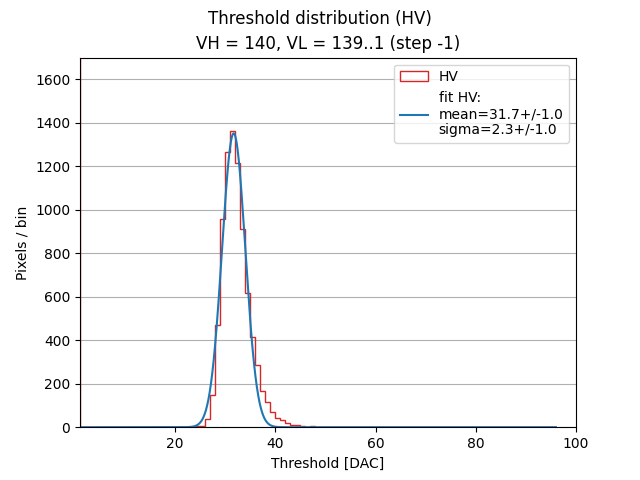
\includegraphics[scale=0.35]{all_HV_thdist_140}}\quad
\subfigure[Noise distribution]
{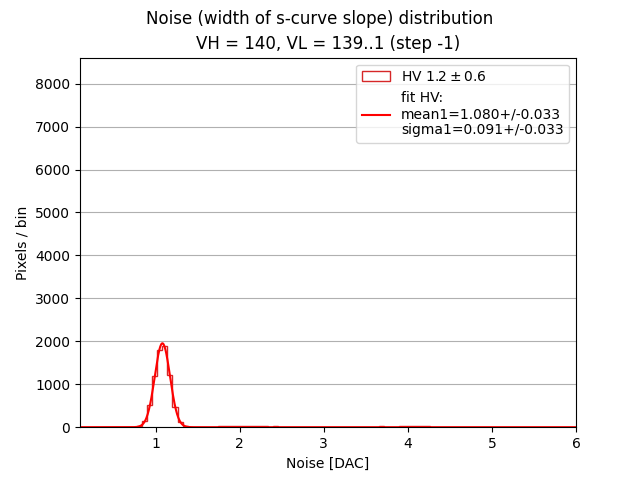
\includegraphics[scale=0.37]{Noise_hist_HV_140_fit}}\\
\caption{HV Normal FE.}
\label{fig:thdist_hv}
\end{figure}


\begin{figure}[h!]
\centering
\subfigure[Threshold map]
{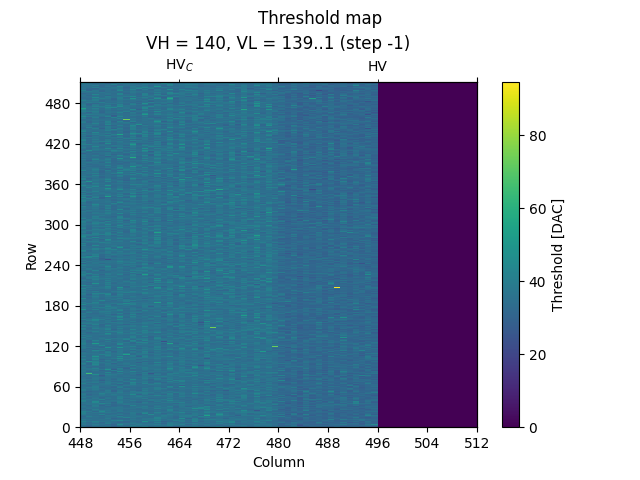
\includegraphics[scale=0.35]{threshold_map_All FEs_140}}\quad
\subfigure[Noise map]
{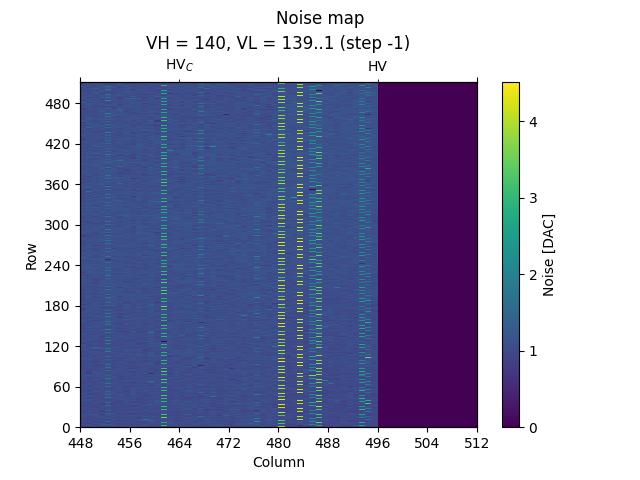
\includegraphics[scale=0.37]{Noise_map_HV Casc._140}}\\
\caption{HV's FE.}
\label{fig:HVs_maps}
\end{figure}

As we will see in the following (\autoref{sec:xtalk}), the atypical s-curves in HVs flavors with many hot pixels, have been the first hint of the cross-talk problem, tied to a global lower threshold in these sectors, compared with the first two threshold measured in the Normal and Cascode sector (with the TB settings). 


\subsubsection{Summary Table}

In~\autoref{tab:th_noise_all} a summary of results for threshold, noise and threshold dispersion of all FE.

\begin{table}[h!]
\centering
\begin{tabular}{>{\columncolor{NavyBlue!70}} c|c|c|c}
\rowcolor{CornflowerBlue}
Front-End & Threshold [DAC] & Threshold dispersion [DAC] & Noise [DAC]\\
\hline
Normal  & 53.62 $\pm$ 0.01 & 2.21 $\pm$ 0.01 & \shortstack{2.503 $\pm$ 0.005 \\ 3.037 $\pm$ 0.002}\\
\hline
Cascode & 60.19 $\pm$ 0.01 & 2.81 $\pm$ 0.01 & 2.400 $\pm$ 0.003\\
\hline
HV - Cascode & 35.34 $\pm$ 0.05 & 2.59 $\pm$ 0.05 & 1.0781 $\pm$ 0.0003\\
\hline
HV & 31.70 $\pm$ 0.10 & 2.30 $\pm$ 0.10 & 1.080 $\pm$ 0.033\\
\hline
\end{tabular}
\caption{Summary table of threshold and noise values for all flavors of the W14R12 chip.}
\label{tab:th_noise_all}
\end{table}

These values measured for threshold, noise and dispersion are much higher than expected in a convenient(useful) working condition (reference table). However, as we have pointed out in the previous, we have carried out the characterization of the matrix response adopting the TB register settings, to obtain results essential for the TB data reconstruction.

In~\autoref{sec:low_thr} we will show some test results, trying to operate the chip at low threshold.



%--------------------------------------------------------------------
\subsection{Threshold dispersion and tuning} \label{sec:tuning}


TJ-Monopix2 is equipped with a circuit which allows the \textit{threshold tuning}. We have already mentioned that the analog part of the in-pixel front-end (\autoref{fig:tj2core}) includes the 3-bit threshold tuning DAC, that can be used to adjust the discriminator threshold of each pixel with respect to the global chip threshold level thus reducing the threshold dispersion. In other words it can adjust every pixel threshold, in order to have a threshold on the matrix as uniform as possible, or in any case a dispersion as small as possible, which is especially important to operate the matrix with low threshold, needed with the reduced collection efficiency due to radiation damage.  This system has been design in order to counteract some negative effects that affect the threshold dispersion like systematics (for example related to biasing), process and temperature variations and radiation damage. \\

Specifically the TDAC circuit, shown in~\autoref{fig:tdac}, helps to make threshold trimming of each pixel. This component controls the discriminator active load current $I_{DISC}$ which is partially responsible of the pixel threshold. It works as an analog multiplexer, which selects one of seven $I_{DISC, n}$ lines generated by the main 8-bit biasing DAC. So the possbile vaue of the final $I_{DISC}$ is given by the sum of two contributions:

\begin{equation}
I_{DISC} = I_{DISC, coarse} + (TCODE - 1) \cdot I_{DISC,fine},  \hspace{.5cm}	where \hspace{.5cm} 1 \leq TDAC \leq 7
\label{eq:tuning_eq}
\end{equation}

\textbf{$I_{DISC, coarse}$} is the current set by the primary value of threshold, resulting by the setting of the main registers which are responsible for it (\autoref{sec:low_thr}). 
\textbf{$I_{DISC, fine}$} is the current selected by the fine tuning step (TDAC) and it depends on the 3-bit tunning code that is stored in the in-pixel configuration memory.
\textbf{TCODE} is the decimal representation of the TDAC code. 

For example if the 3-bit DAC are set to ''111'', the decimal representation is 8 and the fine tuning provide a current $I_{DISC,7}$, which corresponds to the highest threshold. If the 3-bit are set to ''010'' the corresponding TCODE is 2 and the current $I_{DISC,1}$ is provided,  which set the lowest threshold possible around the central value $I_{DISC,coarse}$. The particular combination ''000'' instead (TCODE = 0) masks the single pixel by disabling the discriminator, without affecting the operation of the others.

\begin{figure}
\centering
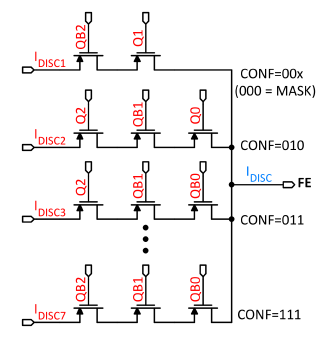
\includegraphics[scale=.8]{tuning_b}
\caption{Schematic of 3-bit tuning DAC (TDAC)}
\label{fig:tdac}
\end{figure}


\subsubsection{First results from threshold tuning}

It has been trying to apply the fine tuning method to level out the threshold of some pixels as much as possible. We have considered about 12.000 pixels of the \textbf{Cascode FE} and in~\autoref{fig:casc_tuning} are shown the results before and after the threshold trimming for the s-curves and threshold distributions.


\begin{figure}[h!]
\centering
\subfigure[Cascode FE s-curves untuned]
{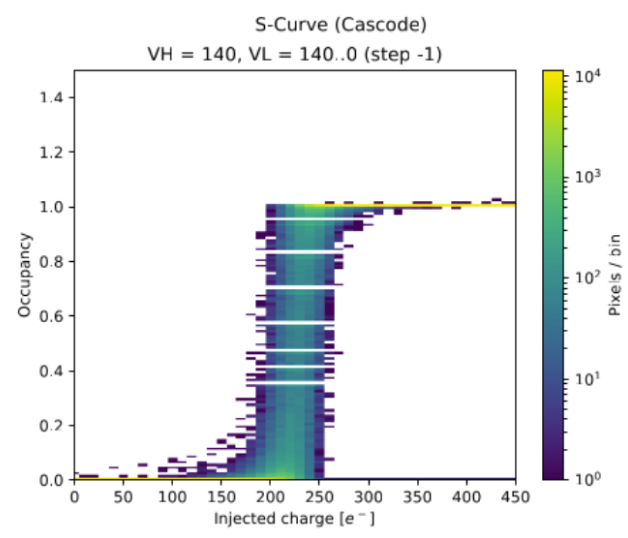
\includegraphics[scale=0.5]{casc_untuned}}\quad
\subfigure[Cascode FE s-curves tuned]
{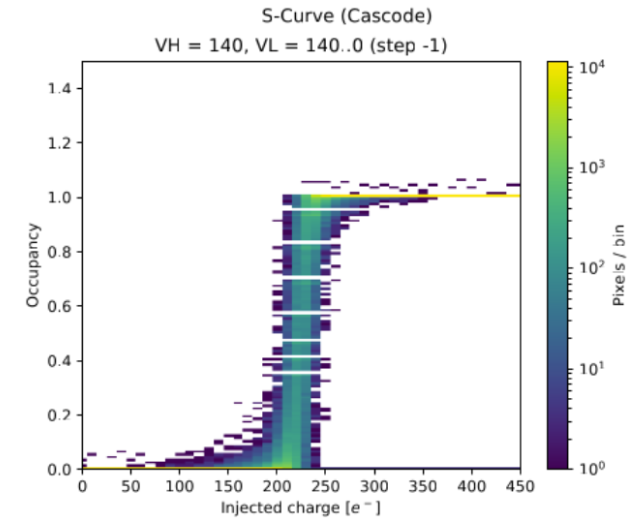
\includegraphics[scale=0.5]{casc_tuned}}\quad
\subfigure[Cascode FE threshold distribution]
{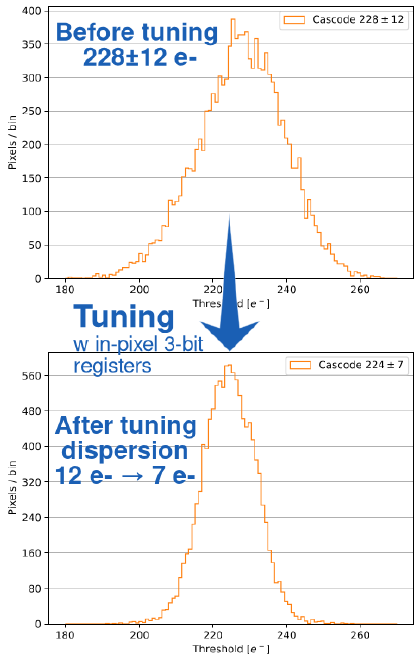
\includegraphics[scale=0.8]{casc_th_tuned_untuned}}\quad
\caption{Cascode FE before tuning and after tuning comparison.}
\label{fig:casc_tuning}
\end{figure}

As we can see the dispersion has been reduced of the 42\% after the tuning and as consequence also the estimation of the threshold is more precise. In~\autoref{fig:casc_maps_tune} are displayed the maps of the threshold and of the TDAC values, such as the value of TCODE assigned at each pixel, in order to obtain a threshold as uniform as possible. \\

\begin{figure}[h!]
\centering
\subfigure[Map of TDAC value with target threshold of $\approx$ 250 $e^{-}$]
{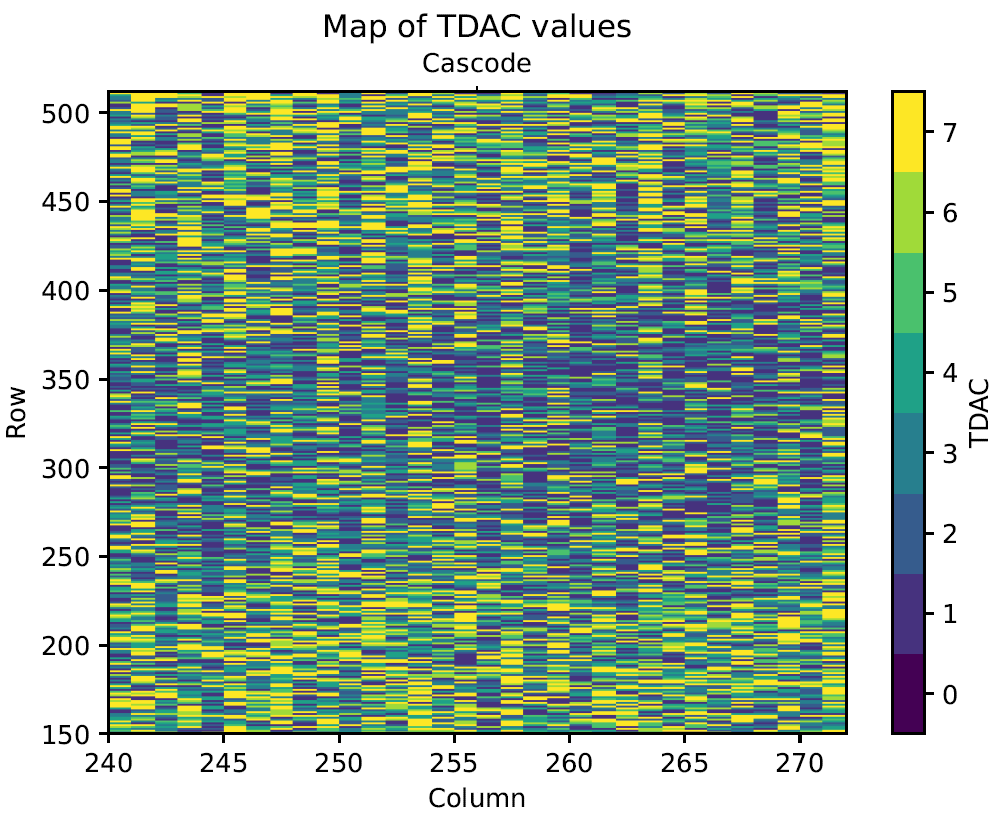
\includegraphics[scale=0.33]{tdac_map}}\quad
\subfigure[Threshold map of tuned Cascode FE]
{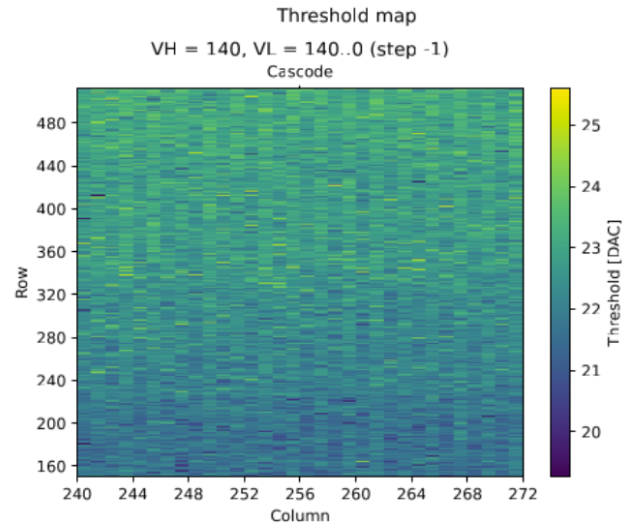
\includegraphics[scale=0.53]{th_map_tuned}}\quad
\caption{Maps of tuned Cascode FE.}
\label{fig:casc_maps_tune}
\end{figure}


%--------------------------------------------------------------------
\section{ToT calibration with internal injection}


The analog information on the signal height is provided by the Time Over Threshold (\autoref{fig:ToT}) digitized with a \SI{25}{ns} clock (BCID clock-frequency is \SI{40}{MHz}). 

\begin{figure}
\centering
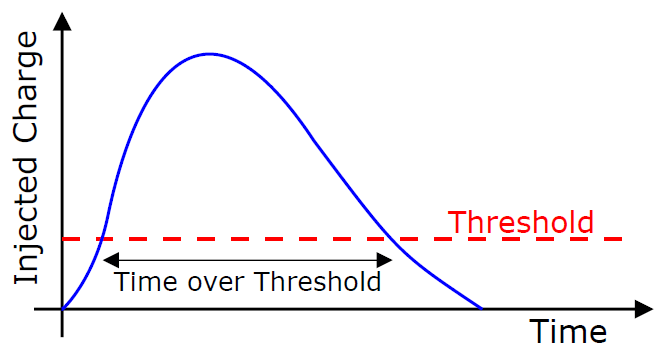
\includegraphics[scale=.7]{ToT3}
\caption{...}
\label{fig:ToT}
\end{figure}

As it has been pointed out in the previous, the choice to use a simple diode instead of a PMOS transistor as reset input baseline element, increases the tolerance to TID radiation but at the same time it implicates a non-linear relationship between the injected charge and the ToT. For this reason, one of the goal of this analysis was to measure the calibration curve ToT vs $Q_{inj}$ via the internal injection. The fit to the calibration curve allows to find the conversion factor needed to reconstruct the signal amplitude. It also allows an absolute calibration of the injection capacitance comparing the results with the ToT response from the radioactive source with known released signal.


%--------------------------------------------------------------------

In carrying out the measurements mentioned above, we started to notice some issues with the injection circuit, which showed some saturation in the voltage pulse at high values of the registers. Due to this issue, the ToT response to internal injection could only be measured up to 170 DAC ($\approx$ 1700 $e^{-}$). This was enough for the absolute calibration using the \ch{^{55}Fe} \SI{5.9}{KeV} line ($\approx$ 1616 $e^{-}$) as explained below.\\

A method has been therefore devised to obtain reliable values of threshold and ToT up to a value of 170 DAC of effective charge injected.\\

The calibration function adopted to describe the $Q_{inj}$-ToT relationship was then used to extrapolate ToT values in the region of high charge (above 170 DAC, $\approx$ 1700 $e^{-}$) not accessible with the injection circuit, to compare with the emission peaks of other radioactive sources and explore a larger range.


%--------------------------------------------------------------------
\subsection{Time Over Threshold (TOT) curves and fit} \label{sec:tot_fit}

The ToT vs $Q_{inj}$ responses for the four flavors of the matrix (using the same TB register settings) are shown in~\autoref{fig:tot_fe}
The function chosen to describe the calibration curves is:

\begin{equation}
y(x) = a\cdot x +b -\frac{c}{x-t}
\label{eq:fit_function}
\end{equation}

with \textit{a}, \textit{b}, \textit{c} and \textit{t} free parameters and where the \textit{y} represents the ToT corresponding to a precise value of collected charge, express by \textit{x}. 

Actually we know that the ToT distribution starts to grow near the threshold, so one of the four free parameters could be computed in function of the threshold value estimated from the previous measurements reported in~\autoref{sec:threshold_subsection}.

In more details, knowing that y($x_{th}$) must be equal to 0 that is the ToT value at the threshold, it can be imposed for example:

\begin{equation}
0 = a\cdot x_{th} + b - \frac{c}{x_{th}-t}  \hspace{.4cm}	\Rightarrow  \hspace{.4cm}	c = x_{th}^{2}\cdot a + x_{th}\cdot (b-a\cdot t) - t\cdot b
\end{equation}

In this way the number of parameters to fit is reduced. In principle a similar equation could be equivalently solved for \textit{a}, \textit{b} and \textit{t}. 

%in turn

Thus different fits have been made: one imposing a constraint on a free parameter (like shown above) and the other one leaving all parameters free. For all of them the value of $\chi^{2}$ (MSE) have been computed and for all flavors it had its minimum when no parameters were fixed. So in the following the results from these last fits with all the parameters left free, have been considered.\\

The same data collected in the previous measurements of thresholds have been used to fit the ToT curves of all pixels for each frontend. As a matter of fact we want to fully characterized the chip response with ''GOE'' settings (\autoref{tab:tb_settings}), in order to use the results to convert ToT to charge collected for the analysis of the TB data.
In~\autoref{tab:th_fe} are reported the results of the fits for all parameters.

\begin{table}[h!]
\centering
\begin{tabular}{c|c|c|c|c}
 & \textbf{Normal} & \textbf{Cascode} & \textbf{HV Cascode} & \textbf{HV} \\
\hline
\hline
\textit{a$\pm\Delta$a [ToT/DAC]} & 0.12$\pm$0.07 & 0.12$\pm$0.01 & 0.257$\pm$0.007 & 0.275$\pm$0.008 \\
\textit{b$\pm\Delta$b [ToT]} & 4$\pm$18 & 1.4$\pm$3.1 & 3.2$\pm$1.4 & 2.3$\pm$1.6 \\
\textit{c$\pm\Delta$c [ToT$\cdot$DAC]} & 200$\pm$1100 & 140$\pm$130 & 160$\pm$70 & 140$\pm$80 \\
\textit{t$\pm\Delta$d [DAC]} & 20$\pm$90 & 40$\pm$15 & 17$\pm$6 & 13$\pm$8 \\
\hline
\hline
\end{tabular}
\caption{Parameters obtained from the fit of ToT curve for each frontend.}
\label{tab:th_fe}
\end{table}

\begin{figure}[h!]
\centering
\subfigure[\textbf{Normal}]
{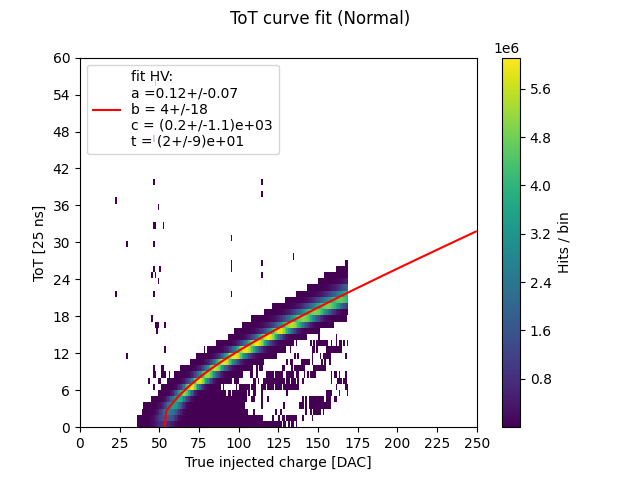
\includegraphics[scale=0.35]{Tot_fit_normal(200)}}\quad
\subfigure[\textbf{Cascode}]
{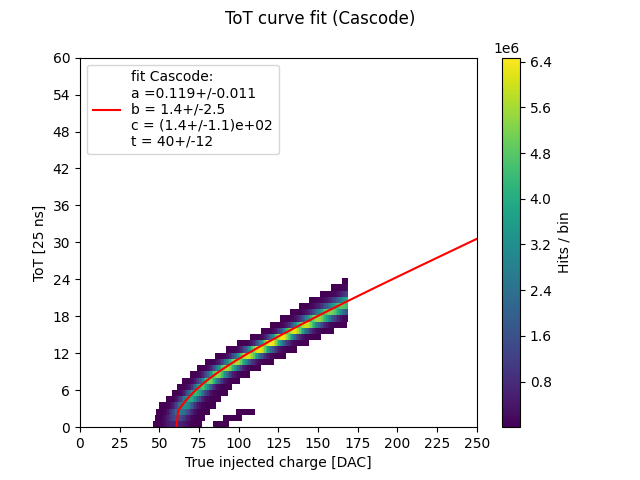
\includegraphics[scale=0.35]{Tot_fit_cascode(200)}}\\
\subfigure[\textbf{HV Cascode}]
{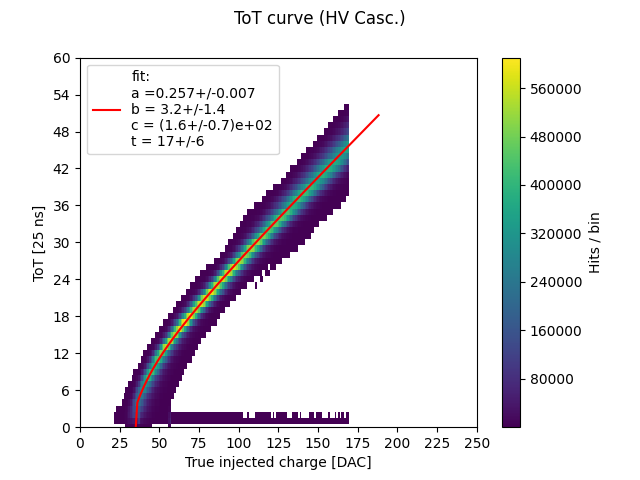
\includegraphics[scale=0.35]{Tot_fit_HV Casc.(200)}}\quad
\subfigure[\textbf{HV}]
{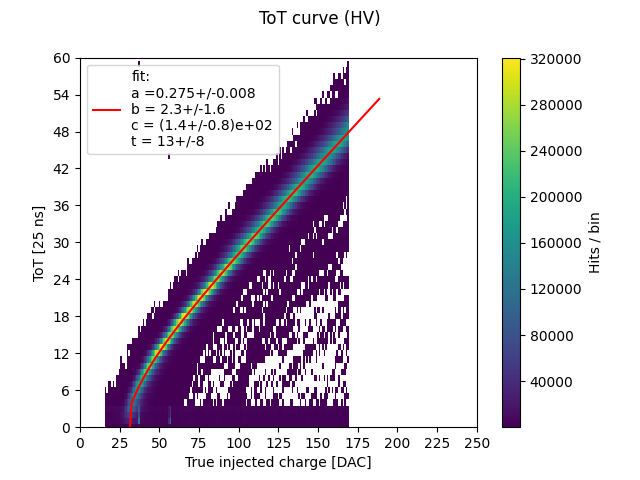
\includegraphics[scale=0.35]{Tot_fit_HV(200)}}\\
\caption{ToT curves fit for all frontend.}
\label{fig:tot_fe}
\end{figure}


%--------------------------------------------------------------------
\section{Response to radioactive source and absolute calibration} \label{sec:source_ana}

%06/10/2022 LOGBOOK

The absolute calibration of the matrix consists in characterizing the response of each pixel to a known signal, like the emission peaks of radioactive sources, then comparing the results with the response from the internal injection circuit to the same amount of charge. By the means of the $Q_{inj}$ - ToT fit (\autoref{sec:tot_fit}), it is possible to convert the ToT signal value to collected charge.\\
Three different X-rays radioactive sources were used to study the signal spectrum of the matrix, with emission lines from 6 to 60 KeV (corresponding approximately to 1600 and 16000 e- respectively).
In fact the knowledge of the sources emission spectrum (in other words, the charge released in the matrix from particles emitted in decays) allows to compare the spectra obtained irradiating the chip, with the expected value of their peaks. It is worth mentioning that only the events in which all charge inducted is collected in a single pixel are part of the peaks reconstructed by the chip.\\
The absolute calibration of the conversion factor of~\autoref{eq:conversion_factor} (i.e. of the injection capacitance $C_{inj}$) is performed with the \SI{5.9}{KeV} peak of the \ch{^{55}Fe} source ($approx$ 1616 $e^{-}$), that is still in the range explored with the injection circuit. The other radioactive sources allowed to extend the ToT comparison at higher values with respect to the limit imposed by the saturation of the internal injection circuit. In~\autoref{tab:radio_sources} are shown the energies of the $\gamma$ emitted by the sources used.\\
Considering that the average energy necessary to produce an electron/hole pair in silicon is 3.65 eV \cite{wermes_book2020}, it is possible to convert the peak energies in a mean value of electrons released using the~\autoref{eq:energy_electron_conv}. So in~\autoref{tab:radio_sources} are reported also the equivalent emission in electrons, which will be useful later.

\begin{equation}
N_{e^{-}} = \frac{E \, [eV]}{3.65 [\frac{eV}{e/h \, pair}]}
\label{eq:energy_electron_conv}
\end{equation}


\begin{table}[h!]
\centering
\begin{tabular}{>{\columncolor{NavyBlue!70}} C{3cm}|C{2.8cm}|C{2.8cm}}
\rowcolor{CornflowerBlue}
Source & Energy $\gamma$ [KeV] & Equivalent charge [$e^{-}$]\\[2ex]
\hline
\ch{^{55}Fe} & 5.9 & 1616\\[0.5ex]
\hline
\ch{^{241}Am} & 13.9 & 3808\\[0.5ex]
\hline
\ch{^{241}Am} & 17.7 & 4849\\[0.5ex]
\hline
\ch{^{241}Am} & 20.7 & 5671\\[0.5ex]
\hline
\ch{^{109}Cd} & 22 & 6027\\[0.5ex]
\hline
\ch{^{241}Am} & 26.4 & 7233\\[0.5ex]
\hline
\ch{^{241}Am} & 59.7 & 16356\\
\hline
\end{tabular}
\caption{Emission lines of \ch{^{55}Fe}, \ch{^{241}Am}, \ch{^{109}Cd} sources visible by the sensor.}
\label{tab:radio_sources}
\end{table}


Now we can go through the results obtained from three different sources: \ch{^{55}Fe}, \ch{^{241}Am} and \ch{^{109}Cd}.
%--------------------------------------------------------------------
\subsection{\ch{^{55}Fe}}

The \ch{^{55}Fe} source decays by \textbf{electron capture} to \ch{^{55}Mn}. One of the photons emitted in this transistion has an energy of 5.9 KeV ($K_{\alpha}$) and it produces via photoelectric effect an electron, which deposits a ionization charge of about 1616 $e^{-}$ in the sensor. 
All flavors were exposed to a \ch{^{55}Fe} source, with activity of \SI{18}{MBq}. In~\autoref{fig:fe_all} are shown the results for the ToT spectrum of single pixels. The peak corresponds to events where the $\gamma$ interacts close to the collection diode and the entire signal is on a single pixel. The shoulder at smaller ToT is due to the charge sharing among several pixels, since no clusters are reconstructed. The peak was fitted by a gaussian function, limited in the region of the peak itself. 

\begin{figure}[h!]
\centering
\subfigure[\textbf{Normal}]
{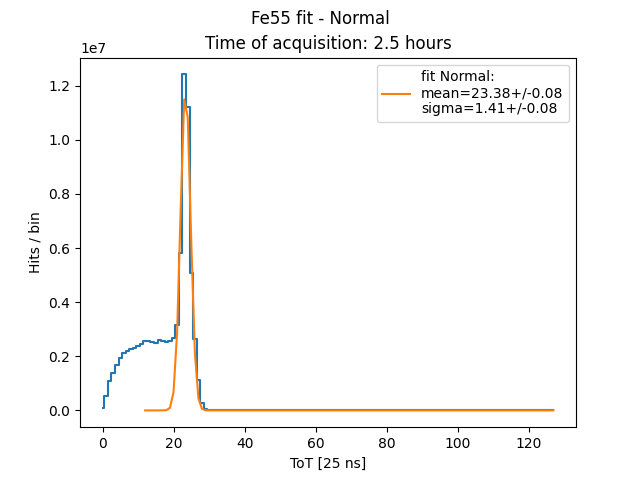
\includegraphics[scale=0.35]{fe55_Normal_peak}}\quad
\subfigure[\textbf{Cascode}]
{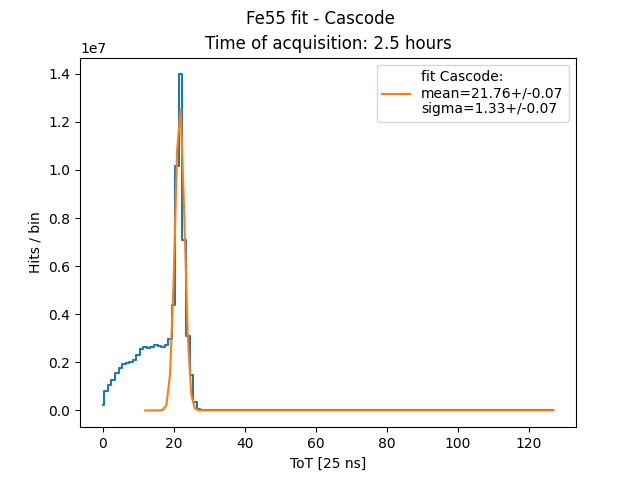
\includegraphics[scale=0.35]{fe55_Cascode_peak}}\\
\subfigure[\textbf{HV Cascode}]
{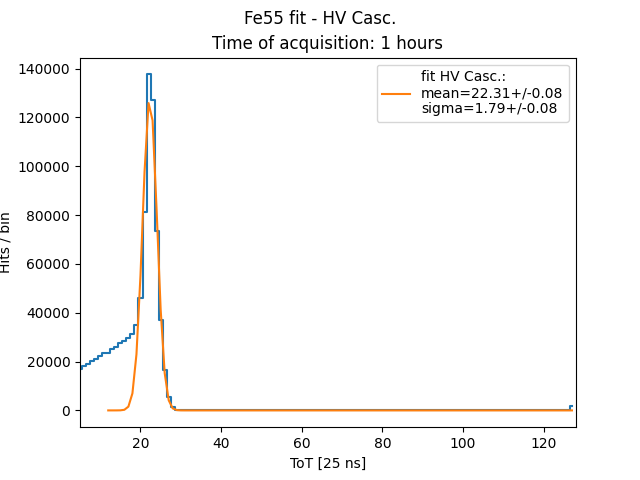
\includegraphics[scale=0.35]{fe_HV Casc._peak}}\quad
\subfigure[\textbf{HV}]
{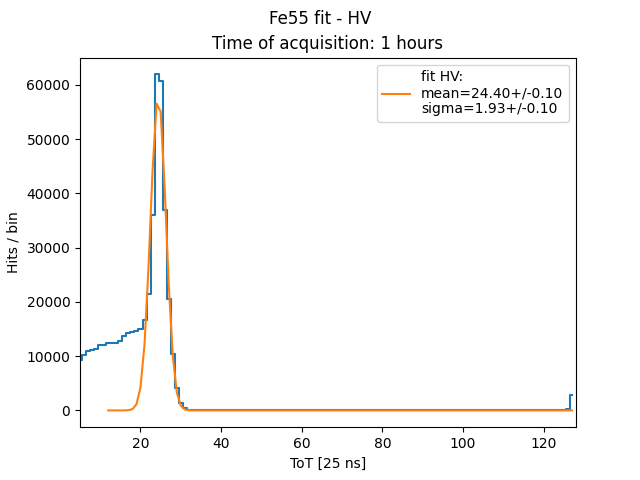
\includegraphics[scale=0.35]{fe_HV_peak}}\\
\caption{\ch{^{55}Fe} peaks for all frontends.}
\label{fig:fe_all}
\end{figure}

As it can be seen for the HV's FE a cut has been applied at low ToT, only to make clearly visible the emission line, since a lot of noisy pixels caused a sharp peak at 0 ToT. In those flavors there were several columns of not-functioning pixels. In the box of each plot are also reported the results of the fit that will be crucial in the following.


%--------------------------------------------------------------------
\subsection{\ch{^{241}Am}}

%AGGIUNGI REFERENZA IMMAGINE (Measurements of gamma-ray emission probabilities of 241, 243Am and 239Np)
%AGGIUNGI REFERENZA (GAMMA RAY SPECTRUM OF AM-241 IN A BACK SCATTERINGGEOMETRY USING A HIGH PURITY GERMANIUM DETECTOR)

The \ch{^{241}Am} source has a more complex spectrum (\autoref{fig:am241_spectrum}) and not all its peaks can be detected by the chip (because of the limited range of ToT available, depending on the numer of bit dedicated to it). The spectrum shows other minor peaks besides the usual intense gamma peaks (59.5 and \SI{26.3}{keV}) and several characteristic L X-rays from \ch{^{237}Np} (20.7, 17.7 and \SI{13.9}{keV}).\\ 

\begin{figure}[h!]
\centering
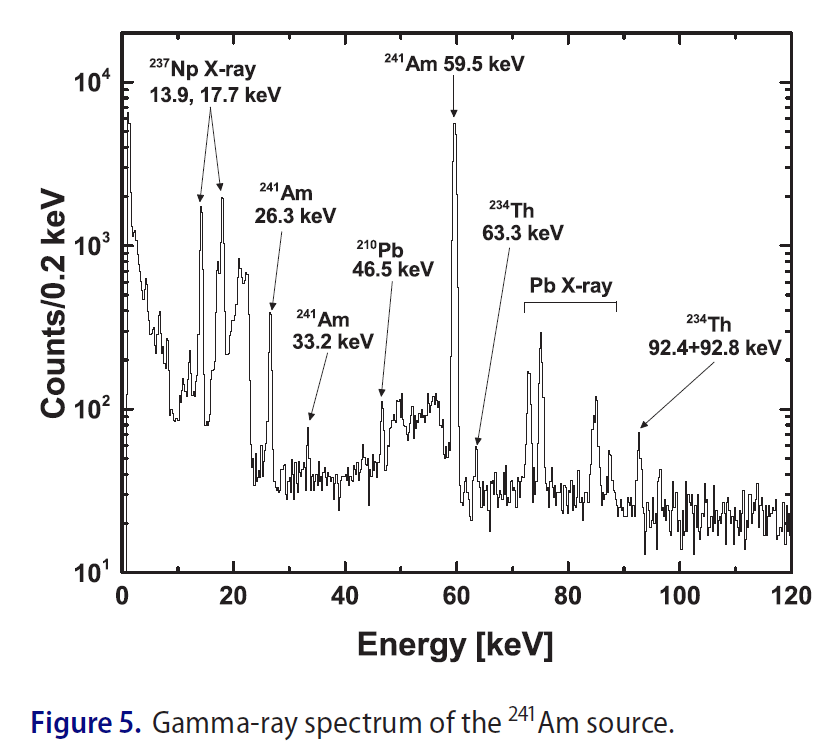
\includegraphics[scale=.4]{Am241}
\caption{\ch{^{241}Am} $\gamma$ emission spectrum.}
\label{fig:am241_spectrum}
\end{figure}

The ToT measured spectra with the \ch{^{241}Am} source on the four flavors are reported in~\autoref{fig:am_all}. Two peaks at lower energy are clearly visible while, for higher ToT values there are larger structures .

\begin{figure}[h!]
\centering
\subfigure[\textbf{Normal}]
{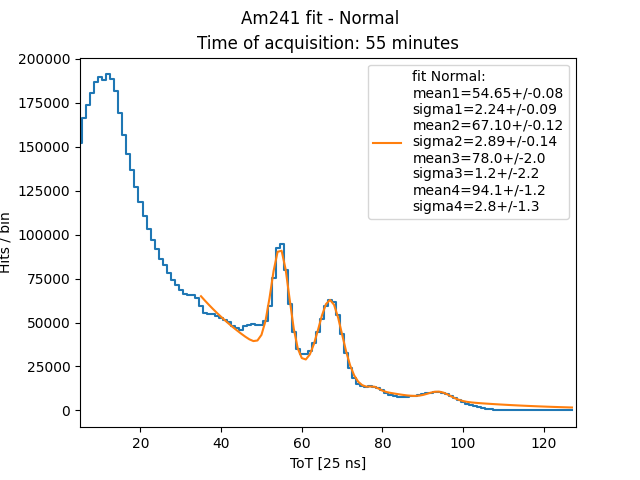
\includegraphics[scale=0.35]{am_Normal_peak}}\quad
\subfigure[\textbf{Cascode}]
{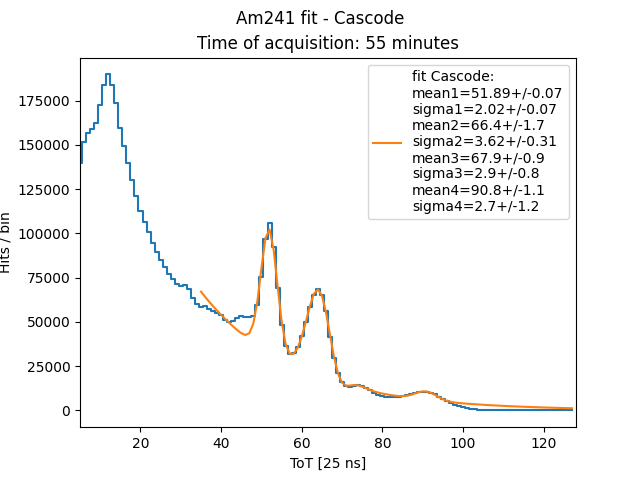
\includegraphics[scale=0.35]{am_Cascode_peak}}\\
\subfigure[\textbf{HV Cascode}]
{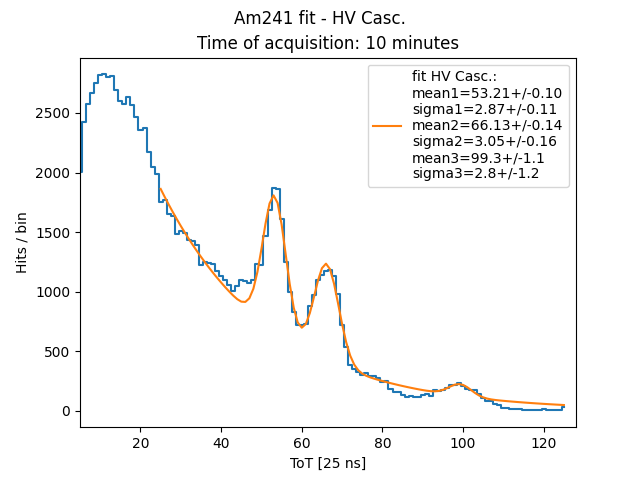
\includegraphics[scale=0.35]{am_HV Casc._peak}}\quad
\subfigure[\textbf{HV}]
{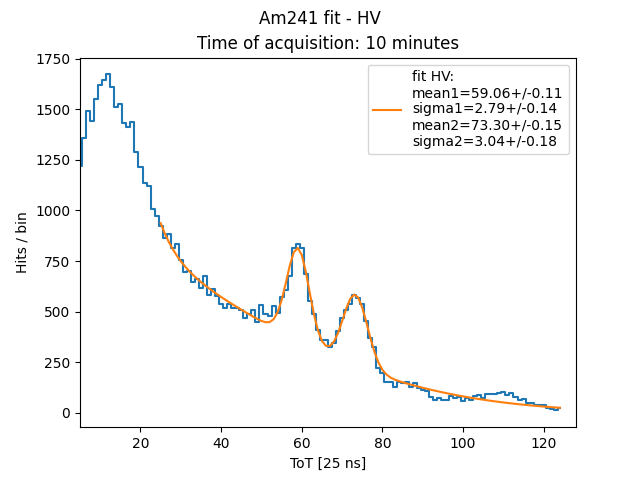
\includegraphics[scale=0.35]{am_HV_peak}}\\
\caption{\ch{^{241}Am} peaks for all frontends.}
\label{fig:am_all}
\end{figure}

In the case of the first two flavors, it could be possible to fit four peaks of the emission lines. In case of the HV's flavors instead, only three peaks for the HV-Cascode FE and two for the HV. As already discussed (\autoref{sec:improved_circuit}) the AC-copuling causes about 41.5\% of signal loss, so they are much less evident and more difficult to fit as isolated peak.


%--------------------------------------------------------------------
\subsection{\ch{^{109}Cd}}

The third source employed was the \ch{^{109}Cd}. This isotope decay in \ch{^{109}Ag} by electronic capture, producing a photon of 22 KeV in the transition. The ToT measured spectra with \ch{^{109}Cd} source on the four flavors of the matrix are reported in~\autoref{fig:cd_all}. 

\begin{figure}[h!]
\centering
\subfigure[\textbf{Normal}]
{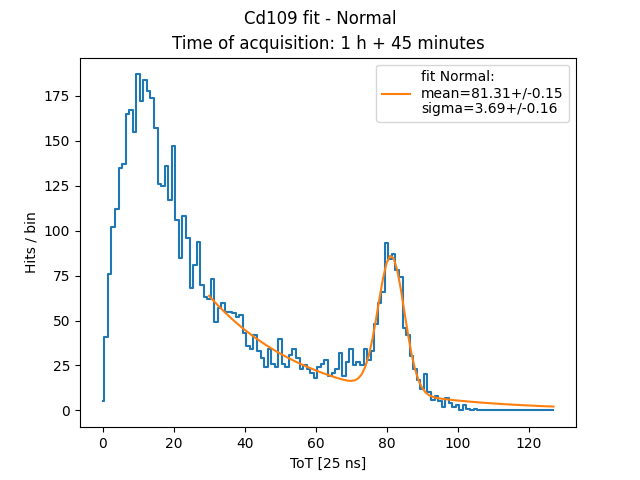
\includegraphics[scale=0.35]{cd109_Normal_peak}}\quad
\subfigure[\textbf{Cascode}]
{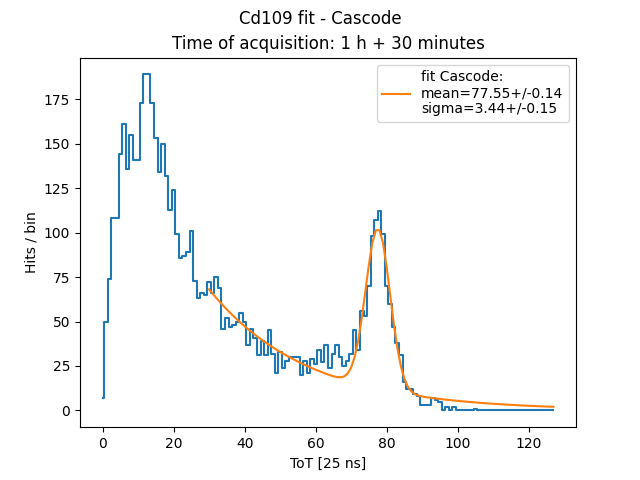
\includegraphics[scale=0.35]{cd109_Cascode_peak}}\\
\subfigure[\textbf{HV Cascode}]
{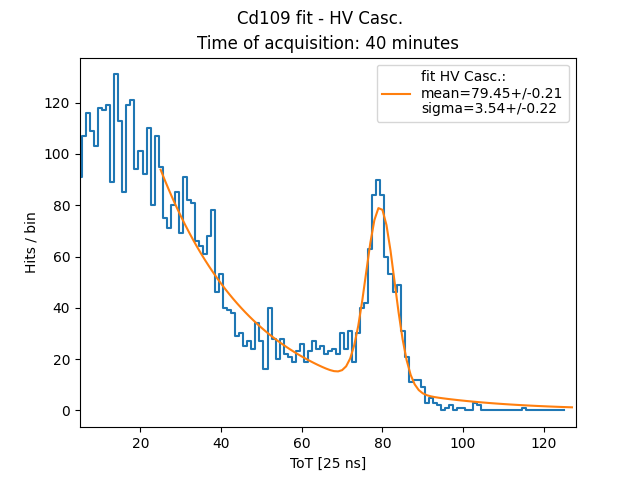
\includegraphics[scale=0.35]{cd109_HV Casc._peak}}\quad
\subfigure[\textbf{HV}]
{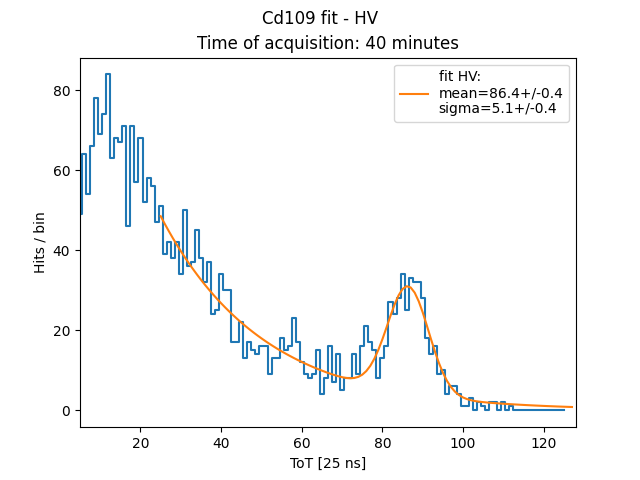
\includegraphics[scale=0.35]{cd109_HV_peak}}\\
\caption{\ch{^{109}Cd} pekas for all frontends.}
\label{fig:cd_all}
\end{figure}

%--------------------------------------------------------------------
%\subsection{\ch{^{190}Sr}}
%%apg 55 tesi


\subsection{Injection capacitance calibration}

%~\autoref{eq:conversion_factor}
The absolute calibration of the conversion factor $K$:

\begin{equation}
K = \frac{C_{inj}}{q_{e^{-}}} \cdot \Delta V_{LSB}
\end{equation}

and of the injection capacitance:

\begin{equation}
C_{inj} = K (\frac{e^{-}}{DAC}) \cdot \frac{\SI{1.6e-19}{\frac{C}{e^{-}}}}{\SI{7.03}{\frac{mV}{DAC}}}
\end{equation}

that convert a signal charge expressed in DAC units to $e^{-}$, is performed using the data from the \ch{^{55}Fe} source. 

As first step the ToT of the peak of the \SI{5.9}{KeV} $\gamma$ line is converted to signal charge in DAC using the fitted calibration curve of~\autoref{eq:fit_function}

Specifically the fit function was inverted obtaining:

\begin{equation}
x(y) = \bigg(\frac{t}{2} - \frac{b}{2a} + \frac{y}{2a}\bigg) \pm \sqrt{\bigg(\frac{t}{2} + \frac{b}{2a} - \frac{y}{2a}\bigg)^{2} + \frac{c}{a}}
\end{equation}

where \textit{x} represents the charge in DAC corresponding to the ToT labeled by \textit{y}.

As shown in~\autoref{tab:radio_sources}, the charge released in the sensor by the \SI{5.9}{KeV} $\gamma$ corresponds roughly to $Q_{\SI{5.9}{KeV}}$($e^{-}$)~=~1616 $e^{-}$. Therefore the conversion factor $K$ for each pixel can be calculated as:

\begin{equation}
K\bigg[\frac{e^{-}}{DAC}\bigg] = \frac{1616 \, e^{-}}{Q_{\SI{5.9}{KeV}}[DAC]}
\label{eq:inj_cap}
\end{equation} 

By these steps, a value of the conversion factor was estimated for each well-functioning pixel. In~\autoref{fig:cap_dist} is reported the distributions of the conversion factor estimated, fitted by a gaussian function.

\begin{figure}
\centering
\subfigure[\textbf{Normal}]
{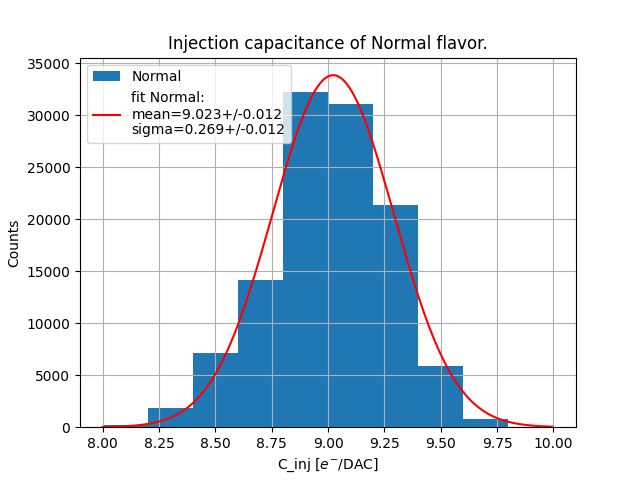
\includegraphics[scale=0.35]{c_inj_alpha_fe_Normal}}\quad
\subfigure[\textbf{Cascode}]
{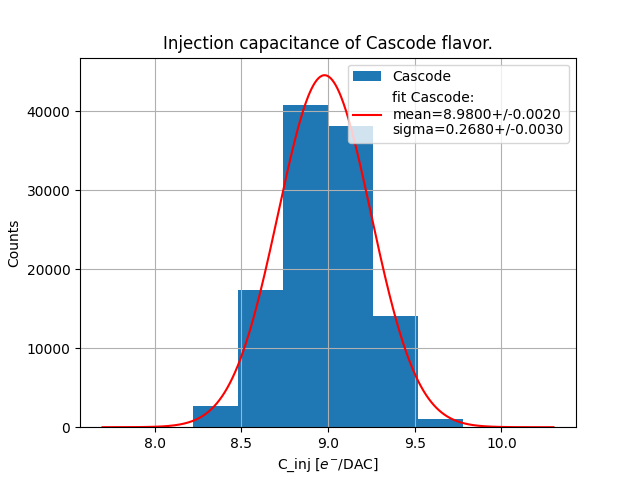
\includegraphics[scale=0.35]{c_inj_alpha_fe_Cascode}}\\
\caption{Injection capacitance distributions of Normal and Cascode FE.}
\label{fig:cap_dist}
\end{figure} 
%%%%%ADD SUMMARY TABLE


\begin{table}[h!]
\centering
\begin{tabular}{>{\columncolor{NavyBlue!70}} C{2.8cm}|C{1.7cm}|C{1.8cm}|C{1.7cm}|C{1.7cm}}
\rowcolor{CornflowerBlue}
Source peak & $K_{Normal}$ ($\frac{e^{-}}{DAC}$) & $K_{Cascode}$ ($\frac{e^{-}}{DAC}$)\\[2.5ex]
\hline
\ch{^{55}Fe} (5.9 KeV) & 9.37 & 9.00\\[1ex]
\hline
\end{tabular}
\caption{Estimation of injection capacitance of Normal and Cascode flavors using the \ch{^{55}Fe} radioactive source emission line at \SI{5.9}{KeV}.}
\label{tab:cap_mean}
\end{table}

\begin{figure}
\centering
\subfigure[\textbf{Normal}]
{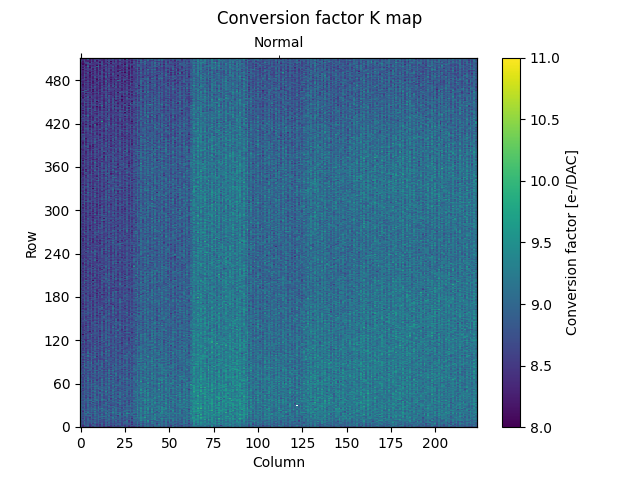
\includegraphics[scale=0.5]{k_maps_Normal}}\quad
\subfigure[\textbf{Cascode}]
{\includegraphics[scale=0.5]{k_maps_Cascode}}\\
\subfigure[\textbf{All}]
{\includegraphics[scale=0.5]{k_maps}}\\
\caption{???}
\label{fig:k_map}
\end{figure} 


%VEDI APPUNTI\\
%We can anyway use these values to interpret data, and also to estimate the charge loss assuming a default conversion factor for all FE.
%%Può parametrizzare perdita di segnale? viene al 51-52% non 40 come previsto.

%[It's necessary to consider that maybe some measurments were done in different conditions of pressure and temperature?]


?????????????
Here it is necessary to point out that for iron source more statistics were collected so in this case a complete analysis of each pixel has been done. For the other sources instead, there weren't enough statistics on every pixel so the injection capacitance has been estimate only as a mean value for the whole front-end, just to compare with the results obtained from the iron analysis.  
In case of \ch{^{55}Fe} source, we managed to fit the emission peak for each working pixel of the whole matrix. 

?????????????

%--------------------------------------------------------------------
\subsection{Check on calibration curve ToT vs $Q_{inj}$ with radioactive sources}

The calibration of the ToT vs $Q_{inj}$(DAC) with the injection circuit could be performed only up to $\approx$ 170 DAC. The radioactive sources can be used up to higher energy to check the agreement with the fitted function in~\autoref{eq:fit_function} .\\
Initially the signal charge in DAC corresponding to each $\gamma$ peak, has been calculated using the nominal conversion factor equal to 10.1 $\frac{e^{-}}{DAC}$. As it could be seen from results in~\autoref{fig:inj_cap_10} there is a reasonable agreement between data and ToT relationship studied in~\autoref{sec:tot_fit}.

After the absolute calibration, assuming the average value of of the conversion factor $K$ (\textit{Mean value}) measured with \ch{^{55}Fe}, the charge in DAC corresponding to the emission peaks have been recalculated and results are shown in~\autoref{fig:inj_cap_sources}.

In~\autoref{tab:source_conv_norm} and in~\autoref{tab:source_conv_casc}   ....(descrizione, specifica quale K usi, richiama tabella?)

\begin{table}[h!]
\centering
\begin{tabular}{>{\columncolor{NavyBlue!70}} C{1.5cm}|C{1.8cm}|C{1.8cm}|C{1.8cm}|C{1.8cm}|C{1.8cm}|C{1.8cm}}
\rowcolor{CornflowerBlue}
Source & Energy $\gamma$ [KeV] & $Q_{expected}$ [$e^{-}$] & $ToT_{measured}$ & $Q_{measured}$ [DAC] & Q [$e^{-}$] \footnotesize{with nominal K factor = 10.1 $e^{-}$/DAC} & Q [$e^{-}$] \footnotesize{with \ch{^{55}Fe} K factor = 9.37 $e^{-}$/DAC}\\[2ex]
\hline
\ch{^{55}Fe} & 5.9 & 1616 & 23.4 & 172 & 1742 & 1616 \\[0.5ex]
\hline
\ch{^{241}Am} & 13.9 & 3808 & 54.7 & 426 & 4304 & 3993 \\[0.5ex]
\hline
\ch{^{241}Am} & 17.7 & 4849 & 67.1 & 529 & 5344 & 4958 \\[0.5ex]
\hline
\ch{^{241}Am} & 20.7 & 5671 & 78.0 & 619 & 6256 & 5804 \\[0.5ex]
\hline
\ch{^{109}Cd} & 22 & 6027 & 81.3 & 647 & 6534 & 6062 \\[0.5ex]
\hline
\ch{^{241}Am} & 26.4 & 7233 & 94.1 & 753 & 7606 & 7057 \\[0.5ex]
\hline
\end{tabular}
\caption{Emission lines of \ch{^{55}Fe}, \ch{^{241}Am}, \ch{^{109}Cd} sources for Normal frontend.}
\label{tab:source_conv_norm}
\end{table}


\begin{table}[h!]
\centering
\begin{tabular}{>{\columncolor{NavyBlue!70}} C{1.5cm}|C{1.8cm}|C{1.8cm}|C{1.8cm}|C{1.8cm}|C{1.8cm}|C{1.8cm}}
\rowcolor{CornflowerBlue}
Source & Energy $\gamma$ [KeV] & $Q_{expected}$ [$e^{-}$] & $ToT_{measured}$ & $Q_{measured}$ [DAC] & Q [$e^{-}$] \footnotesize{with nominal K factor = 10.1 $e^{-}$/DAC} & Q [$e^{-}$] \footnotesize{with \ch{^{55}Fe} K factor = 9.00 $e^{-}$/DAC}\\[2ex]
\hline
\ch{^{55}Fe} & 5.9 & 1616 & 21.8 & 180 & 1813 & 1616 \\[0.5ex]
\hline
\ch{^{241}Am} & 13.9 & 3808 & 51.9 & 427 & 4316 & 3846 \\[0.5ex]
\hline
\ch{^{241}Am} & 17.7 & 4849 & 66.4 & 549 & 5540 & 4937 \\[0.5ex]
\hline
\ch{^{241}Am} & 20.7 & 5671 & 67.9 & 561 & 5667 & 5050 \\[0.5ex]
\hline
\ch{^{109}Cd} & 22 & 6027 & 77.6 & 642 & 6483 & 5777 \\[0.5ex]
\hline
\ch{^{241}Am} & 26.4 & 7233 & 90.8 & 753 & 7604 & 6776 \\[0.5ex]
\hline
\end{tabular}
\caption{Emission lines of \ch{^{55}Fe}, \ch{^{241}Am}, \ch{^{109}Cd} sources for Cascode frontend.}
\label{tab:source_conv_casc}
\end{table}


%SPIEGATABELLAAA

As we can see, a better agreement is therefore obtained and this shows that through calibration we are now able to interpret data with greater precision, which was the main purpose of this analysis.

\begin{figure}
\centering
\subfigure[\textbf{Normal}]
{\includegraphics[scale=0.35]{ToT_Normal_thesis}}\quad
\subfigure[\textbf{Cascode}]
{\includegraphics[scale=0.35]{ToT_Cascode_thesis}}\\
\caption{ToT of all flavors assuming the nominal(expected) conversion factor equal to 10.1 $\frac{e^{-}}{DAC}$.}
\label{fig:inj_cap_10}
\end{figure} 


\begin{figure}[h!]
\centering
\subfigure[\textbf{Normal}]
{\includegraphics[scale=0.35]{ToT_Normal_iron}}\quad
\subfigure[\textbf{Cascode}]
{\includegraphics[scale=0.35]{ToT_Cascode_iron}}\\
\caption{ToT linearity of all flavors assuming the conversion factor obtained from \ch{^{55}Fe}.}
\label{fig:inj_cap_sources}
\end{figure} 




%--------------------------------------------------------------------
\section{Operation with low threshold} \label{sec:low_thr}

One of the most important target in sensor design is to keep high efficiency even after irradiation damages. All experimental environments indeed, are exposed to high doses of radiations, so it's crucial to ensure the functionality of the detectors, even after being irradiated.

For this reason, many tests were done in order to understand the chip behaviour at low threshold where a good value of efficiency could be preserved.
Moreover working at low threshold allows to detect low charge events due to charge sharing or charge trapping (effect which increases after irradiation), expecially in case of thin epitaxial material. 


%--------------------------------------------------------------------
\subsection{Register optimization}

As we have seen in section (REFERENCE), there are a lot of registers which control the discriminator threshold and also the readout sequence. So preliminary it was necessary to explore their possible settings in order to operate the chip at low threshold.\\

Now we will go through the main registers used for this purpose, in order to explain their functionality. There are several dozens of registers but we focused on some of the most important and crucial to set the threshold and its dispersion.

\begin{itemize}
\label{currents}
\item \textit{$I_{CASN}$} : this current is responsible of the output baseline signal. In particular it sets the baseline of the FE output that goes to the input discriminator. In a few words, higher this value, higher the baseline, lower the threshold and also a little bit the gain and vice versa by decreasing it.
\item \textit{$I_{THR}$}: it controls the pre-amplifier feedback strenght and speed, so it is responsible for the output reset rate. Increasing this current increases the gain and the time that the analog output takes to get back to the baseline and as consequence, it increases a lot the maximum value of the ToT. In fact it is recommend to set $I_{THR}$ to low value (e.g. 8 nA[ref]) in order to avoid high ToT slope.
\item \textit{$I_{DB}$}: this current corresponds to \textbf{$I_{DISC,coarse}$} explained in~\autoref{sec:tuning}. It represents the primary current that sets the discriminator threshold, to which another current is added by the the tuning.
\item \textit{$I_{TUNE}$}: it corresponds to \textbf{$I_{DISC,fine}$} instead (\autoref{sec:tuning}). Remembering the equation from tuning \footnote{
\begin{equation}
I_{DISC} = I_{DISC, coarse} + (TCODE - 1) \cdot I_{DISC,fine},  \hspace{.5cm}	where \hspace{.5cm} 1 \leq TDAC \leq 7
\end{equation}
} (\autoref{eq:tuning_eq}), this is the current to multiply by the TDAC value, which is added to $I_{DB}$, during the tuning process.
\item \textit{$I_{BIAS}$}: this current acts on the pre-amplifier input transistor and influences the threshold dispersion and the gain. In particular increasing this value, the dispersion decreases and the gain becomes greater. Nevertheless it can't be increased a lot because it affects the power consumption, too. %higher rise time? pre-ampl output rise time??
%\item \textit{$V_{RESET}$}: this register influences the threshold dispersion. Lowering its value, the dispersion decreases and vice versa
\end{itemize}

\begin{comment}
pag.97 tesi
This modification has significant consequences in several design aspects such as the bandwidth, gain, noise and threshold dispersion resulting in a different front-end behavior
\end{comment}

%ITHR : on chat hung said instead ITHR=64 corresponds to 25 nA and ITHR=20 to 8 nA
%https://confluence.desy.de/pages/viewpage.action?spaceKey=BI&title=VTX+Lab+Set+Up+Operation

%--------------------------------------------------------------------
\subsection{Comparison between data and simulation}

In the interest of understanding how the registers' setting of the chip influences the threshold, several measurements have been taken with different configuration of their values.
The results are compared with simulations done by Hung Pham.  (...). [???]

\begin{description}
\item[\textbf{$I_{CASN}$}] 
\end{description}

In figure \vref{fig:icasn_sim}, we can see the simulated behaviour of the threshold and the gain, increasing the value o $I_{CASN}$.

\begin{figure}[h!]
\centering
\includegraphics[scale=.8]{thr_gain_icasn(sim)}
\caption{Trends of Gain and Threshold increasing $I_{CASN}$.}
\label{fig:icasn_sim}
\end{figure}

\begin{figure}[h!]
\centering
\includegraphics[scale=.5]{all_trends(ICASN)}
\caption{Threshold vs. $I_{CASN}$ for $I_{THR}$= 20, 40, 64.}
\label{fig:alltrends_icasn}
\end{figure}

To verify the trend of threshold as this current varies, three different acquisitions have been taken by fixing $I_{THR}$ = 20, 40, 64 and increasing $I_{CASN}$ from 0  to 30 DAC, with a step of 5 DAC. We have done this enabling 200 pixels in the Cascode FE (rows: 472 - 512, cols: 225 - 230).[??]\\

Each threshold distribution has been fitted with a gaussian function in order to estimate the average threshold value and its dispersion.

In figure \vref{fig:alltrends_icasn} are reported all trends obtained.


\begin{description}
\item[\textbf{$I_{THR}$}]
\end{description}

Reusing the same data of the previous measurements, the trend of the threshold have been studied bt changing the value of $I_{THR}$ and fixing that of $I_{CASN}$. In this case only $I_{CASN}$ from 0 to 15 DAC is considered, because for higher values we don't have enough measures of the threshold (specifically only two for $I_{THR}$=40, 64). The results are shown in figure \vref{fig:alltrends_ithr}.

\begin{figure}[h!]
\centering
\includegraphics[scale=.5]{all_trends(ITHR)}
\caption{Threshold vs. $I_{THR}$ for $I_{CASN}$= 0, 5, 10, 15.}
\label{fig:alltrends_ithr}
\end{figure}

As expected, increasing $I_{THR}$ results to lower gain and faster return to baseline, so higher threshold. 
We can compare them with the simulation shown in figure \vref{fig:ithr_sim}. 

\begin{figure}[h!]
\centering
\includegraphics[scale=.6]{ithr_simulation}
\caption{Trends of Gain and Threshold increasing $I_{CASN}$.}
\label{fig:ithr_sim}
\end{figure}

\begin{description}
\item[\textbf{Time over Threshold (ToT)}]
\end{description}

The last analysis done to make a comparison with the simulations, is about the trend of the ToT changing the value of $I_{CASN}$ for a fixed value of $I_{THR}$ and vice versa. In particular we consider the data obtained with $I_{CASN}$ fixed to 0 DAC and $I_{THR}$ to 64 DAC, which are the values studied and used for these registers during the Test Beam in Desy.

\begin{figure}[h!]
\centering
\subfigure[ToT vs $I_{THR}$ ($I_{CASN}$=0 DAC) - Data (\textbf{Cascode})]
{\includegraphics[scale=0.45]{tot_curves_icasn0}}\quad
\subfigure[ToT vs $I_{THR}$ ($I_{CASN}$=0 DAC) - Simulation]
{\includegraphics[scale=0.5]{tot_curves_icasn0_simu}}\\
\caption{ToT vs $I_{THR}$}
\label{fig:tot_vs_ithr}
\end{figure}

\begin{figure}[h!]
\centering
\subfigure[ToT vs $I_{CASN}$ ($I_{THR}$=64 DAC) - Data (\textbf{Cascode})]
{\includegraphics[scale=0.5]{tot_curves_ithr64}}\\%\quad
\subfigure[ToT vs $I_{CASN}$ ($I_{THR}$=64 DAC) - Simulation]
{\includegraphics[scale=0.35]{tot_curves_ithr64_simu}}\\
\caption{ToT vs $I_{CASN}$}
\label{fig:tot_vs_icasn}
\end{figure}

Results are reported in~\autoref{fig:tot_vs_ithr} and~\autoref{fig:tot_vs_icasn}. Also here we can see a good agreement between data and simulations.

%--------------------------------------------------------------------
\subsubsection{some nice picture of the optimized thr and tuning}

!!!!


\section{Cross talk issue and mitigation} \label{sec:xtalk}

As it was already pointed out, during the measurements of the average threshold of all FEs, there were something atypical in the s-curves of the HV flavors (subsection \vref{first_xtalk}), indeed some pixels seem to have occupancy greater than 1. This behavior threatens the good functionality of the overall matrix response, because these \textit{noisy pixels} flood the readout, giving unreliable results.

Also the systematic study of different register configurations has revealed the presence of the hot pixels which prevent to use certain settings and as consequence to reach lower global thresholds. \\

For this reason an investigation has been conducted in order to understand the reasons why they start to fire and how to cure them as far as possible.
In the meantime an important issue with cross-talk of the readout signals was discovered, and so in this section we examine this effect and some attempts to mitigate it using different settings/bias.


\subsection{Hot pixel issue}

First of all we noticed that in the s-curves oh the HV flavors (e.g. that of HV-Cascode reported in figure \vpageref{fig:hot_first}), the atypical behavior could be triggered by a digital signal sent to the matrix during the readout activity at low threshold. This consideration is based on two main reasons:

\begin{itemize}
\item when the matrix has high threshold, like for Normal and Cascode FE, all pixels seem to behave as expected, without \textit{hot pixels}.\\ Lowering the threshold and running some source acquisitions without any source, no strange behaviour was observed. Acquiring data with a radioactive source instead, even Normal and Cascode FE seem to reveal the same problem. This led to thinking that during the readout of good pixels an induced signal is created which couples with some other pixels, in particular with those at lower threshold with respect to the average value. If the height of this signal exceeds the threshold of the single pixel, it causes some spurious hits, making the pixel ''\textbf{hot}''.

\item Moreover, always considering the HV Cascode s-curves, it could be noticed that in the region before the threshold ($Q_{inj}$<threshold, pointed by the blue arrow) there isn't an anomalous activity which means that the induced signal is not due to the BCID tha is always sent to the matrix during the injection or an acquisition with the source, regardless of being above or below the  threshold. The atypical behaviour indeed, is in the region above the threshold ($Q_{inj}$>threshold, pointed by the red arrow) where the occupancy of some pixels becomes greater than 1. This means that these \textit{hot pixels} detect more hits of those injected.

\end{itemize} 

\begin{figure}[h!]
\centering
\includegraphics[scale=.5]{hot_first_HV}
\caption{HV-Cascode s-curves.}
\label{fig:hot_first}
\end{figure}

From these first observations, we have reached the conclusion that the cross talk could be tied to the readout activity. So we have started investigating the timestamp of those hits not synchronize with the timestamp of the injection.


\subsection{Hot pixel strategy (study)}

At first, it has been lowered the threshold in order to ''create'' hot pixel also in the first two flavors of the matrix. In fact with TB settings the threshold was too high and the hypothetical induced signal did not cause sporious hits. For this purpose different settings were tried, changing some fundamental registers responsible for the threshold like those listed and explained \vpageref{currents}. 

Then several tests have been run under controlled conditions:
\begin{itemize}
\item one healty(good) pixel was injected;
\item one \textit{hot pixel} (two or three in different tests) was enabled but not injected;
\item the all matrix except these pixels was disabled.
\end{itemize}

In this way (remembering the readout sequence [REFERENCE]) the readout cycle has a known duration and two different timing info has been used to study the induced signal with greater precision:

\begin{itemize}
\item \textbf{$\Delta$TS} (TimeStamp) between two consecutive hits: the TimeStamp is assigned from the FPGA when the \textsc{token} rises on the TE of the first hit to read, but only if the previous readout frame is completed. So, if the hit coming from a \textit{hot pixel} is after the hit from the injected one, the minimum $\Delta TS$ has to be equal to the readout time of 1 pixel and so to the duration of the \textsc{FREEZE\_STOP} signal .\\
This info has allowed to verify if the hot pixel fires after the good injected one or not.
\item LE(hit) - TE(previous hit): this quantity measures the elapsed time between a hit and the previous one. This is a finer info than the $\Delta$TS because it allows to correlate the hit with the induced digital signal, originate from the readout cycle.
\end{itemize}

Moreover, since a 7-bit BCID is sent to the matrix during its activity, it was important to keep short (<128 clock cycle) the duration of the full readout sequence and to not enable too many pixels in order to not extend too much the readout frame. Otherwise the information on the leading edge of the pixel could not be correlated with the token of the previous hit. In other words, if the readout frame exceed 128 clock cycles, since the token could be raised if the matrix is \textbf{not} freeze, even if an hit is arrived before it could be read only in the next frame when it could rise again the token, but in this case it will have different TimeStamp. So in this case the TS is useless for our purpose.


\subsection{Cross-talk (Results)}

Referring to the readout sequence, in order to understand which signal could induce cross talk, each register value has been moved one by one.
In table \vpageref{tab:ro_registers} just an example from the several settings tried is reported.

\begin{table}[h!]
\centering
\begin{tabular}{>{\columncolor{ForestGreen!60}} C{5cm}|C{1.7cm}}
\rowcolor{PineGreen!80}
Register & Value \\
\hline
\textsc{FREEZE\_START\_CONF} & 10\\[0.3ex]
\hline
\textsc{READ\_START\_CONF}& 13 \\[0.3ex]
\hline
\textsc{READ\_STOP\_CONF} & 15 \\[0.3ex]
\hline
\textsc{LOAD\_CONF} & 30 \\[0.3ex]
\hline
\textsc{FREEZE\_STOP\_CONF} & 31\\[0.3ex]
\hline
\textsc{STOP\_CONF} & 31\\[0.3ex]
\hline
\end{tabular}
\caption{Register values of the Readout cycle.}
\label{tab:ro_registers}
\end{table}

Doing so indeed, the LE-TE info has to shift by the same value with which the signal that cause the cross talk has been changed. This step of the procedure is tied with the necessity to keep the readout sequence within the maximum 128 BCID range.\\

For example, if \textsc{FREEZE\_START\_CONF} is responsible for the cross talk signal, we expct that shifting its value by a certain amount, the hot pixels start to fire after that this signal arises due to the hit on the injected pixel. So the value of LE-TE has to be \textsc{FREEZE\_START\_CONF} + some potential delay. Same argument for the other registers. \\

By this procedure, repeated for each readout register, we have come to the conclusion that the cross-talk could be related to the raising and falling edge of the \textsc{FREEZE} signal.

In figure \vpageref{fig:xtalk} an example of some results obtained. It is the histogram of the time last between the leading edge of an hit and the trailing edge of the previous hit, when one pixel is injected and two are read. It's possible to see several peaks (reffering to the readout setting reported in table \vpageref{tab:ro_registers}):

\begin{itemize}
\item one at 0, that represent the situation in which both hits come from hot pixel firing simultanously after the injection. This means that they are activated by the same signal and so it is the most important confirmation that is cross-talk and not random firing pixel signal;
\item one at $\approx$ 18 equal to \textsc{FREEZE STAR} raising + 8 $\rightarrow$ first induced signal;
\item one at $\approx$ 35 equal to \textsc{FREEZE STOP} falling + 4 $\rightarrow$ second induced signal;
\item one at $\approx$ 55 equal to \textsc{FREEZE STOP} falling + 4 when two different pixels are read. In more details, after the first 30 time unit until the first \textsc{LOAD CONF}, a distinct pixel reading starts and it takes another 20 time unit (\textsc{LOAD} - \textsc{FREEZE START}) + 1 unit time to conclude the frame with the \textsc{FREEZE STOP} and so 51 + 4 unit time wrote above. Therefore when two pixels are read, the \textsc{FREEZE STOP} falls after 51 clock cycles, and it is compatible with the last peak in the plot.
\end{itemize}

%%ReFIRING???

\begin{figure}[h!]
\centering
\subfigure[An example of the time quantity used in the analysis.]
{\includegraphics[scale=0.8]{xtalk_time}}\quad
\subfigure[An example of the LE(hit)-TE(previous hit) histogram.]
{\includegraphics[scale=0.4]{xtalk_hist}}\\
\caption{Some results of the cross-talk studies.}
\label{fig:xtalk}
\end{figure}

As already stated, we run several tests varying the number of pixels to read, the value of the readout registers, different combination of hot and good pixels and also different spatial location of them in the matrix to exclude the possibility that the problem was related to particular columns. All results are in agreement with the interpretation explained above.\\

?????...\\
Furthermore it hase been tried to estimate the height of the induced signal from the threshold of the hot pixel. For this reason we have have tried different setting of the currents cited above to make a pixel \textit{hot} in order to understand when the induced signal went above the threshold. We have found that the signal could (may) correspond to 100/150 $e^{-}$.\\
??????
%the height of the cross talk signal from FREEZE was measured lowering gradually the THR of good pixels to monito when they become hot.

In figure \vpageref{fig:analog_xtalk} an analog acquistion of the readout signals taken by an oscilloscope.


\begin{figure}
\centering
\includegraphics[scale=.6]{xtalk_analog}
\caption{Cross-talk of the \textsc{FREEZE} signal on oscilloscope's analog output, for different value of \textsc{FREEZE\_START\_CONF} register.}
\label{fig:analog_xtalk}
\end{figure}

In these tests one pixel was injected from 0 to 140 DAC (in the acquisition it can be seen in the increasing signal height). There are two different group of spikes: the first which is smaller and represent the cross-talk from the raising of the \textsc{FREEZE} signal and the second, larger and corresponding to the cross talk from the falling edge of the same signal.
Moreover it's possible to see that in the two different pictures, the cross talk signals move according to the different settings of the \textsc{FREEZE START/STOP} edge.

%meglio una lista??


\subsection{Mitigation}

As seen in the previous, the problem of the hot pixel is tied to the induction signal produced during the readout, which cause cross-talk. It becomes even more serious when there is a grater dispersion threshold.\\

Potentially every pixel could become \textit{hot} if its threshold is lower than the height of the cross-talk signal, since the \textsc{FREEZE} in sent across the entire matrix. 

As an example, in figure \vpageref{fig:making_hot} it si possible to compare the behaviour of pixel (218, 123) for different register settings adopted in order to reduce the threshold.

\begin{figure}[h!]
\centering
\subfigure[$I_{DB}$=100, $I_{TUNE}$=53 - Good behavior (the red one)]
{\includegraphics[scale=0.35]{making_hot1}}\quad
\subfigure[$I_{DB}$=60, $I_{TUNE}$=150 - Pixel starts to misbehave]
{\includegraphics[scale=0.35]{making_hot3}}\\
\subfigure[$I_{DB}$=55, $I_{TUNE}$=150 - Pixel becomes \textit{hot}]
{\includegraphics[scale=0.35]{making_hot2}}\\
\caption{S-curve of the pixel (218, 123) for different register settings.}
\label{fig:making_hot}
\end{figure}

 
\begin{description}
\item \textbf{Threshold trimming}
\end{description}
 
Therefore a possible treatment could be related to the threshold tuning, explained in section (\vref{tuning}) , which could allow to make the pixel threshold more uniform (less threshold dispersion) and simultanously to target a value greater than the induced signals. \\

In figure \vpageref{fig:tuning_hot} an example of the results obtained.

\begin{figure}
\centering
\subfigure[Threshold distribution before tuning procedure.]
{\includegraphics[scale=0.3]{before_tuning}}\quad
\subfigure[Threshold distribution after tuning procedure.]
{\includegraphics[scale=0.3]{after_tuning}}\\
\caption{Threshold tuning to reduce hot pixels.}
\label{fig:tuning_hot}
\end{figure} 

It' evident the reduction of the tail in the threshold distribution, in fact the dispersion is reduced by 56\%. Also the hot pixels decrease from 18\% to 1.2\% of the total number of pixels studied. We can also notice that the peak at 0 threshold disappears.

%It was effectively done managing to obtin lower threshold
%DEVI METTERE ESEMPIO???
%DAC tuning kaje threshold more uniform, threat hot pixel and so also the peak at zero tot in source acquisition is reduced

\begin{description}
\item \textbf{Bias Voltage}
\end{description}

Moreover it has been tried to increase the voltage bias of the all matrix, too. We remember that all previous test has been run with $P_{WELL}/P_{SUB}$ set to -3 V. This value was increased to -6 V and indeed there were some improvements. In fact increasing the bias, we expected a decrease of the diode capacitance thus higher gain and lower thresold dispersion. In addition the coupling with the cross talk signal is reduced too and so the induced signal height. \\
In figure \vpageref{fig:bias_comp} a comparison between the threshold distribution respectively at -3 V and -6 V, with same registers setting and without tuning.

\begin{figure}[h!]
\centering
\subfigure[Threshold distibution at $P_{WELL}/P_{SUB}$=-3 V.]
{\includegraphics[scale=0.3]{th_dist_3V}}\quad
\subfigure[Threshold distibution at $P_{WELL}/P_{SUB}$=-6 V.]
{\includegraphics[scale=0.3]{th_dist_6V}}\\
%\caption{}
\label{fig:bias_comp}
\end{figure}

At higher bias voltage not only is the threshold lower (higher gain), but also its dispersion, as expected. And despite that there are fewer hot pixels: 1.3\% at -6V against 17\% at -3 V. Also here there is clear a reduction of the threshold distribution tail. 

\subsubsection{Final results?}

Eventually the final results obtained with both threshold tuning and a bias voltage on $P_{WELL}/P_{SUB}$=-6 V. 

\begin{figure}[h!]
\centering
\subfigure[Threshold distibution at $P_{WELL}/P_{SUB}$=-6 V without tuning.]
{\includegraphics[scale=0.3]{xtalk_6V_no_tuning}}\quad
\subfigure[Threshold distibution at $P_{WELL}/P_{SUB}$=-6 V with tuning.]
{\includegraphics[scale=0.3]{xtalk_6V_tuning}}\\
%\caption{}
\label{fig:bias_tuning}
\end{figure}

As we can see in figure \vpageref{fig:bias_tuning}, the threshold dispersion decreases together with the number of the hot pixels. In fact without the tuning, there are 1.3\% of them, instead with tuning procedure there are none at all.



%LOWERING ITHR DECREASED THE INDUCED SIGNAL, BUT MATRIX NOT GOOD FUNCTIONALITY?
%VRESET(agisce sulla dispersione) AND IBIAS(aumenta gain e diminuisce dispersion ma aumenta power consumption)



\begin{comment}
Suggestions from OBELIX meeting.

Probably the coupling is linked to digital power. 
Not from the bulk: +4 clk seems to be the indication for not a direct coupling

Since the distribution of the power is from the edge,  first and last column should be more solid against this effect and hot pixel should be more present in the center? 
They asked if we have a  map of the hot pixels

Also suggested to change the clock and see if the delay from the FREEZE edge is at the same delay or not. 

\end{comment}



\section{Test Beam results}

This full characterization of the chip allowed to interpret data collected during the Test Beam done in Desy in June 2022. Several measurements have been taken, among which: pixel response, noise level, cluster signal, full depletion depth, voltage scan and angular scan. In particular the aim was to study electrical characteristics and hit detection effciency of unirradiated modules.



\subsection{Experimental apparatus and DUTs }

The measurements have been performed in a 4 (o 5) GeV electron beam at DESY II testbeam facility at DESY, Hamburg. The experimental apparatus consisted of a beam telescope, a Trigger Logic Unit to provide trigger and control signals employed during test beams, a scintillator trigger and a rotation-translation stage on which install the device under test. (figure \vpageref{fig:tb}).

\begin{figure}[h!]
\centering
\includegraphics[scale=.7]{TBJUNE22_2}
\caption{Test Beam experimental apparatus.}
\label{fig:tb}
\end{figure}



\begin{comment}
\begin{figure}[h!]
\centering
\subfigure[Test beam apparatus.]
{\includegraphics[scale=0.8]{TBJUNE22_PHOTO}}\quad
\subfigure[Test beam schematics.]
{\includegraphics[scale=0.8]{TBJUNE22}}\\
\caption{Test Beam setting at DESY.}
\label{fig:tb}
\end{figure}
\end{comment}

Three different modules have been tested with different sensor geometry, among which the chip W14R12 that we have studied in depth through laboratory measurements. All results described in previous sections have been crucial to interpret data obtained during these tests.

In the following we will briefly mention the results obtained.


\subsection{Hit detection efficiency measurements}

Initially a depletion depth study have been done and with a voltage bias of -3 V (Normal and Cascode FE), for the chip W14R12 resulted 33$\mu$m $\pm$ 0.04 (stat.) $\pm$ 2.53 (sys.).

Voltage scan measurements have been performed for both the two type of pixel couplings, such as DC and AC coupled. For the latter, only some first results have been obtained. 

\begin{description}
\item[Normal FE]
\end{description}

In figure \vpageref{fig:tb_NF} are reported results obtained for \textbf{Normal FE} of all modules. As expected, efficiency and clusters grow as the bias voltage is increased. 

\begin{figure}[h!]
\centering
\includegraphics[scale=.7]{tb_NF_res}
\caption{Cluster size and efficiency results for Normal FE.}
\label{fig:tb_NF}
\end{figure}


\begin{description}
\item[Cascode FE]
\end{description}

Same trends for \textbf{Cascode FE} are shown in figure \vpageref{fig:tb_CASC}.

\begin{figure}[h!]
\centering
\subfigure
{\includegraphics[scale=0.8]{tb_CASC_cluster}}\quad
\subfigure
{\includegraphics[scale=0.8]{tb_CASC_eff}}\\
\caption{Cluster size and efficiency results for Cascode FE.}
\label{fig:tb_CASC}
\end{figure}


In particular in figure \vpageref{fig:tb_DC_Cz} are reported the hit map efficiency for DC-coupled pixels for the W14R12 chip, which includes Normal and Cascode FE.

\begin{figure}[h!]
\centering
\includegraphics[scale=.7]{tb_DC_eff}
\caption{Efficiency for DC-coupled pixel of W14R12 chip: (99.79 $\pm$ 0.10) \%}
\label{fig:tb_DC_Cz}
\end{figure}



\begin{description}
\item[HV Casc. FE]
\end{description}

\begin{figure}[h!]
\centering
\includegraphics[scale=.7]{tb_HVC_res}
\caption{Cluster size and efficiency results for HV Cascode FE.}
\label{fig:tb_HVC}
\end{figure}


\begin{description}
\item[HV FE]
\end{description}

\begin{figure}[h!]
\centering
\includegraphics[scale=.7]{tb_HV_res}
\caption{Cluster size and efficiency results for HV FE.}
\label{fig:tb_HV}
\end{figure}































%%%%%%%%%%%%%%%%%%%%%%%%%%
%			BIBLIOGRPAHY
%%%%%%%%%%%%%%%%%%%%%%%%%%

%1. THESIS MUSTAKAS
%2. GAMMA RAY SPECTRUM OF AM-241 IN A BACK SCATTERING GEOMETRY USING A HIGH PURITY GERMANIUM DETECTOR (for Am241) 
%KOLANOSKI per converision factro 3.65
%CDR
%articoli giuliana
